\documentclass[a4paper,openany,12pt]{book}
\usepackage{graphicx}
\usepackage[spanish,mexico]{babel}
\usepackage[utf8]{inputenc}
\usepackage{sty/fancyhdr}
\usepackage{ae}
\usepackage[left=2.5cm,right=2.5cm,top=3cm,bottom=2cm]{geometry}
\usepackage[printonlyused]{acronym}
\usepackage{xspace}
\usepackage{flafter}
\usepackage{sty/hlundef}
\usepackage{sty/tesis}
\usepackage{setspace}
\usepackage{amsmath}
\usepackage{algorithm2e}
\usepackage{natbib}
\setcitestyle{numbers,notesep={: }}
\usepackage{tabularx}
\newcolumntype{Y}{>{\centering\arraybackslash}X}

\title{Ensamble de múltiples subconjuntos de datos balanceados aplicado a puntuación crediticia}

\author{Carrillo Pino, José Enrique}

\advisor{Prof. DSc. Dennis Barrios Aranibar}

\examinerone{Prof. Dr. Hidalgo Buena Gente}{Presidente}%
\examinertwo{Prof. Dr. Manuel Armando Líos}{Vocal}%
\examinerthree{Prof. Dr. Antero A. Gal Oppe}{Secretario}%
\examinerfour{Prof. Dr. Casso E. Staria}{Externo}{Universidad del ABC} % of being the case
%\date{30 de Junio del 2018}
\date{\today}

\dedicado{Dedico este trabajo a mis padres que me encaminaron hasta aquí, a mis profesores que me aportaron los conocimientos necesarios y a mi pareja amigos y pareja que influyeron de forma positiva en mi vida para hacerme la persona que soy ahora.}

\begin{document}
\pagestyle{fancy}

\maketitle %Compone la carátula y la dedicatoria
\newpage

\approved{\cuatro}%  {\tres} or {\cuatro}

%mayores detalles de como usas las abreviaturas (acronimos)
% vea: http://www.ctan.org/tex-archive/macros/latex/contrib/acronym/
% hay un manual en pdf en esa misma direccion

\chapter*{Abreviaturas}

\begin{acronym}

% Classification algorithms
\acro{ECDD}{Ensamble de Clasificadores para Datos Desbalanceados}
\acro{LR}{Logistic Regression}
\acro{MLP}{Multi Layer Perceptron}
\acro{DBN}{Deep Belief Network}
\acro{RBM}{Restricted Boltzman Machine}
\acro{SVM}{Support Vector Machine}
\acro{CSVM}{Clustered Support Vector Machine}
\acro{LS-SVM}{Least Squares Support Vector Machine}
\acro{AD}{Árbol de Decisión}
\acro{RF}{Random Forest}
\acro{XGBoost}{eXtreme Gradient Boosting}
\acro{LDA}{Linear Discriminant Analysis}

% Evaluation metrics
\acro{ROC}{Receiver Operating Characteristic}
\acro{TPR}{True Positive Rate}
\acro{AUC}{Área Under the Curve}
\acro{PR}{Precision-Recall Curve}
\acro{AP}{Average Precision}

% Other
\acro{ReLU}{Rectified Linear Units}
\end{acronym}


\begin{agradecimientos}

En primer lugar deseo agradecer a mis padres por el apoyo brindado y su preocupación de encaminarme bien en la vida, con una rica educación tanto académica como en valores.

Agradezco a la universidad, mi alma matter, por haberme cobijado y brindado la formación que ahora me permitirá ayudar a construir una mejor sociedad.

Agradezco de forma muy especial a mi asesor Prof. DSc. Dennis Barrios por haberme guiado en esta tesis.

Deseo agradecer de forma especial a mis profesores: Ernesto Cuadros, Yván Túpac y José Peñarrieta porque fueron ejemplos que deseo seguir en mi vida profesional.

Y finalmente agradezco a mi pareja y amigos que fueron una influencia muy positiva a lo largo del estudio de mi carrera profesional.

\end{agradecimientos}
 %Inserta los agradecimientos
\begin{resumen}
La investigación actual en puntuación crediticia no ha prestado atención al desbalanceo presente en los conjuntos de datos. Por esta razón, en este trabajo se importó un método reciente de ensamble para clasificar datos desbalanceados en el dominio de crédito. Se usaron cuatro clasificadores base de diversas familias, y tres datasets heterogéneos como prueba. Luego de ejecutar los experimentos, los resultados son bastante alentadores; el poder predictivo mejoró para todos los clasificadores base. Además, los clasificadores ensamblados creados superaron por un poco a los algoritmos del estado del arte Random Forest y XGBoost. Finalmente, al comparar nuestros resultados con los resultados de otros estudios en dos datasets benchmark se ratifica que los resultados son bastante competitivos.
\end{resumen}
 %Inserta el resumen
\begin{abstract}
Current credit scoring research does not exploit the feature of the datasets of being of an imbalanced nature. For this reason, in this work, a recent bagging method for imbalanced data was imported to the credit scoring domain. Four base classifiers of different families and three heterogeneous datasets were used as evidence. After running the experiments, the results are quite encouraging; the area under de curve (AUC) improved for ten out of twelve base classifiers. In addition, the created bagging classifiers were statistically superior than the modern bagging classifiers Random Forest and XGBoost. Finally, we compare the results with the results of other studies of the state of the art in two benchmark datasets, confirming that the results are quite competitive.
\end{abstract} %Inserta el abstract

\pagenumbering{roman}
\setcounter{page}{1}
\pagestyle{plain}

\tableofcontents %Inserta el índice general
\listoftables %Inserta el índice de cuadros
\listoffigures %Inserta el índice de figuras

%%%%%%%%%%%%%%%%%%%%%%%%%%%%%%%%%%%%%%%%%%%%%%%%%%%%%%%%%%%%%%%%%%%%%
%%%%   En esta parte deberas incluir los archivos de tu tesis   %%%%%
%%%%%%%%%%%%%%%%%%%%%%%%%%%%%%%%%%%%%%%%%%%%%%%%%%%%%%%%%%%%%%%%%%%%%

\pagestyle{plain}
\pagenumbering{arabic}
\setcounter{page}{1}
\chapter{Introducción}

El área de Aprendizaje Automático es muy fructífera y cuenta con abundante investigación. Uno de los objetivos de esta área es resolver problemas de clasificación, es decir, dadas un conjunto de características observadas, asignar una categoría basado en ejemplos vistos anteriormente. Estos algoritmos clasificadores son entrenados mediante algoritmos de aprendizaje supervisados.

Un problema de clasificación que tiene solamente dos categorías es llamado binario. Una de las aplicaciones en el mundo real de estos clasificadores binarios se halla en el área de calificación crediticia, donde la tarea es clasificar a las personas en buenos y malos pagadores, basandose en el historial de crédito y otras variables de comportamiento que cada entidad financiera pueda recolectar.

Al utilizar los algoritmos de aprendizaje automático en problemas de calificación crediticia, habilitamos una poderosa herramienta que podría mejorar las tasas de interés a las que son ofrecidas los préstamos e incrementar la inclusión financiera a nivel global.

\section{Motivación y Contexto}

El momento en que se publica este trabajo es muy emocionante, puesto que en el entorno emprendedor peruano han surgido varias \textit{Fintech} (entidad que brinda servicios financieros basados en innovación tecnológica) que aprovechan el potencial del aprendizaje automático para expandir el porcentaje de la población que tiene acceso al crédito, que actualmente está rondando el 30\%.

Las instituciones financieras tradicionales se han dado cuenta de esto y también están empezando a utilizar herramientas de aprendizaje automático para mantenerse competitivas.

Desde el lado de la ciencia, este florecimiento del campo de aplicación ha impulsado la investigación en esta área, de modo que ahora tenemos nuevos algoritmos poderosos y eficientes como \ac{XGBoost} \citep{Chen:2016:XST:2939672.2939785} y nuevas técnicas de \textit{bagging} (entrenamiento de varias instancias del modelo con diferentes subconjuntos de la base de datos).

Sin embargo, cuando se aplican estas técnicas, muchas veces se olvidan características intrínsecas de los datos en esta área, lo que lleva a crear modelos subóptimos. De ahí surge la necesidad de enfocarnos en estas características particulares para mejorar el estado del arte existente.

\section{Planteamiento del Problema}

% Donde y cuando aparece el problema? A quien afecta?
Al entrenar modelos para predecir morosidad, los conjuntos de datos siempre son desbalanceados. Esto ocurre en todas las entidades financieras del mundo. El desbalance puede encontrarse desde un moderado 30\% hasta llegar a menos de 1\% de instancias de la clase minoritaria, que suelen ser los créditos morosos.

% Qué intentos ha habido de solucionar el problema?
Se ha intentado solucionar este problema haciendo sobremuestreo y submuestro. También se ajustan los parámetros de los modelos para compensar el desbalance. Pero estos métodos aún no han tenido un efecto significativo en el poder predictivo de los modelos.

% Qué pasa si no se soluciona el problema?
Los modelos de crédito ineficientes perjudican a las entidades financieras y los prestatarios. Las entidades financieras tienen elevadas tasas de morosidad y costos elevados de adquisión de clientes. Mientras que los prestatarios encuentran más caro y mas difícil acceder a un crédito.

% El problema tiene implicaciones más amplias?
% Cuál es la relevancia cokmputacional
Resolver este problema podría mejorar el acceso al crédito para muchas personas, especialmente en nuestro país Perú, donde el 70\% de la población aún no está bancarizada. Y desde el punto de vista computacional, permitiría encontrar nuevas aplicaciones para las técnicas de aprendizaje de máquina para conjuntos de datos desbalanceados.


\section{Objetivos}

Aplicar en el área de calificación crediticia, un reciente método de ensamble para clasificación de datos desbalanceados \citep{sun2015novel}. Y compararlo con otros modelos del estado del arte.


\subsection{Objetivos Específicos}

\begin{itemize}
	\item Implementar el método de ensamble para poder realizar pruebas con él.

	\item Elegir 3 bases de datos para ejecutar los experimentos.

	\item Comparar el desempeño de cuatro clasificadores: (\ac{LR}, \ac{MLP}, \ac{SVM} y \ac{AD}); contra su versión ensamblada. Para comprobar si el ensamble mejora el poder predictivo de estos clasificadores base.

	\item Comparar el desempeño de los cuatro clasificadores ensamblados en el punto anterior contra otros algoritmos de ensamble del estado del arte: \ac{RF} y \ac{XGBoost}. Para comprobar si es un método de ensamble al menos competitivo.

	\item Comparar el desempeño de los cuatro clasificadores ensamblados, con los resultados de otros trabajos de investigación del estado del arte, usando conjuntos de datos de referencia. De esta manera verificar si hay una mejora respecto al estado del arte.
\end{itemize}

\section{Organización de la tesis}

En el capítulo 2 se dará un marco teórico al mismo tiempo que una revisión del Estado del Arte. Se abordarán temas como la historia de la minería de datos y los puntajes de crédito, estudios comparativos y problemas identificados con la investigación actual. También explicaremos los algoritmos de clasificación usados en esta investigación, los algoritmos de ensamble referenciales, el algoritmo de ensamble para datos desbalanceados y los algoritmos de evaluación. Finalmente se hará un estudio del trabajo relacionado.

En el capítulo 3 se explicarán los experimentos llevados a cabo en esta investigación. Se hablará de los conjuntos de datos utilizados, la metodología seguida y los procesos mediante los cuales se lograron los objetivos y se obtuvieron los resultados.

Luego en el capítulo 4 se presentarán los resultados de este trabajo en forma de tablas, al mismo tiempo que se harán algunos comentarios sobre observaciones interesantes y conclusiones relevantes.

Finalmente en el capítulo 5 se bosquejan las conclusiones, problemas encontrados, recomendaciones y se proponen trabajos futuros.

%\section{Cronograma}

%Esta sección sólo es para aquellos alumnos que estén presentando su plan de tesis. Esta sección no va en la tesis final.
 %Inserta el capítulo 1
\chapter{Estado del Arte en Calificación Crediticia}

La calificación crediticia se obtiene mediante un conjunto de modelos de decisión que ayudan a los prestamistas a otorgar créditos. Estas técnicas son usadas para decidir quién obtiene crédito, cuánto crédito deben obtener, a qué precio lo tendrán, y qué estrategias operacionales mejorarán la rentabilidad de los clientes. Un puntaje de crédito puede ser transformado en la probabilidad del cliente de no pagar el préstamo. Así, desde el año 2000, se ha convertido en un pilar de los modelos desarrollados por instituciones financieras cumplir los requerimientos del Acuerdo de Basilea que dictamina que se deben estimar las probabilidades de morosidad de cada portafolio de préstamos \citep[1]{thomas2017credit}.

Con los avances en minería de datos y Big Data, ahora hay calificaciones crediticias siendo desarrolladas usando fuentes alternativas de datos. Estas pueden ser psicométricas, datos ``sociales'' en línea, o datos del teléfono móvil. Sin embargo, a parte de la consideración de por qué esta información debería ser predictiva del comportamiento crediticio, hay una mayor incertidumbre respecto al hecho de quiénes realmente poseen este tipo de información \citep[18]{thomas2017credit}.

Algunos desafíos claramente identificados en la creación de calificaciones crediticias están relacionados con la disponibilidad de los datos, su exactitud y su confiabilidad \citep[18--19]{thomas2017credit}. Sin embargo no trataremos estos temas porque están fuera del ámbito de esta investigación.

Cuando los puntajes de crédito se desarrollaron por primera vez en los años 1950s y 1960s, los únicos métodos utilizados fueron de discriminación estadística. Aún hoy, con el advenimiento de muchos nuevos enfoques de clasificación basados en minería de datos, los métodos estadísticos, especialmente la regresión logística son por mucho los métodos más utilizados para construir calificaciones crediticias \citep[25]{thomas2017credit}. Tienen la ventaja de permitir el uso de herramientas como los intervalos de confianza y prueba de hipótesis en el contexto de calificación crediticia. Así, uno es capaz de comentar el poder discrimatorio del modelo construido y la importancia relativa de la diferentes características (variables) que constituyen el modelo y su discriminación. De esta forma, uno es capaz de usar esta información para proponer cambios en las preguntas hechas a los prestatarios.

Actualmente numerosas técnicas de clasificación han sido adoptadas para hacer calificación crediticia. Estas técnicas incluyen métodos estadísticos (e.g. análisis discrimante y regresión logística), modelos estadísticos no paramétricos (e.g. K-nearest neighbour y árboles de decisión) y redes neuronales. Con frecuencia surgen conflictos cuando se comparan las conclusiones de algunos de estos estudios. Por ejemplo, en \citep{desai1996comparison} encontraron que las redes neuronales se desempeñan considerablemente mejor que el análisis discriminante al predecir los malos préstamos, mientras que \citep{yobas2000credit} reportó que el segundo supera al primero. Por esto, el problema de escoger una técnica de clasificación para hacer la calificación crediticia permanece como una problema difícil y desafiante \citep{baesens2003benchmarking}.

Los últimos estudios comparativos en esta área son del año 2003 \citep{baesens2003benchmarking} y 2015 \citep{lessmann2015benchmarking}. En el último estudio comparativo de 2015 se compararon 41 métodos de clasificación a través de 8 conjuntos de datos. Además se creó una tabla muy interesante \citep{lessmann2015benchmarking} comparando los algoritmos de clasificación y evaluación utilizados en los últimos estudios. En dicha tabla se evidencia que los algoritmos más utilizados son las \ac{MLP}, las \ac{SVM} y métodos de ensamble. También se ve que los algoritmos de evaluación más utilizados son el \ac{AUC} y aquellos que involucran un umbral, como error de clasificación, \ac{TPR}, etc. También se incluye información sobre qué estudios utilizaron una validación estadística de la hipótesis.

A pesar de tener mucha investigación, la literatura sobre calificación crediticia no refleja varios recientes avances en aprendizaje predictivo \citep{lessmann2015benchmarking}. Estos avances conciernen 3 dimensiones:

\begin{itemize}
    \item Nuevos algoritmos de clasificación
    \item Nuevas medidas de desempeño para \textit{evaluar} modelos
    \item Pruebas de hipótesis estadísticas para \textit{comparar} modelos 
\end{itemize}

Un análisis de le literatura de modelamiento de morosidad confirma que los estudios en esta área tienen varias limitaciones \citep{lessmann2015benchmarking}:

\begin{itemize}
    \item Utilizan pocos o pequeños conjuntos de datos
    \item No comparan diferentes clasificadores de estado del arte entre ellos
    \item Usan un pequeño conjunto de indicadores de exactitud conceptualmente similares
\end{itemize}

A continuación se dará un breve repaso de los algoritmos que se utilizarán en esta investigación, tanto para la clasificación como para la evaluación de los modelos.

\section{Algoritmos de clasificación base}
%En random forest hay que poner la diferencia con decision tree. %https://towardsdatascience.com/the-random-forest-algorithm-d457d499ffcd

\subsection{Regresión Logística}

Es un modelo estadístico que, en su forma básica, utiliza una función logística para modelar una variable binaria dependiente. A continuación la definición formal.

Dado que $y\in \{0, 1\}$ y $\vec{x}$ sea el vector de entrada, se tiene un vector de parámetros $\vec{w}$ y un intercepto $w_0$. Para clasificar a $\vec{x}$ se calcula una combinación lineal de $\vec{x}$ y $\vec{w}$, a la que luego se le aplica la función logística para obtener la probabilidad de que $y = 1$, tal como se muestra en la fórmula \ref{eq:lr}.

\begin{equation}
    \label{eq:lr}
\begin{split}
    f(\vec{x}) &= w_0 + \vec{w}\cdot\vec{x} \\
    P(y=1|\vec{x}) &= \frac{1}{1 + \exp(-f(\vec{x})) }
\end{split}
\end{equation}

\subsection{Multi Layer Perceptron}

El modelo de Multi Layer Perceptron es la red neuronal más utilizada. Está inspirada por el funcionamiento del cerebro humano. Típicamente, se compone de tres capas, una capa de entrada, una capa de neuronas ocultas y una capa de salida. Cada neurona procesa su entrada y genera una salida que es transmitida a las neuronas en la siguiente capa.

\begin{figure}[htbp]
    \centering
    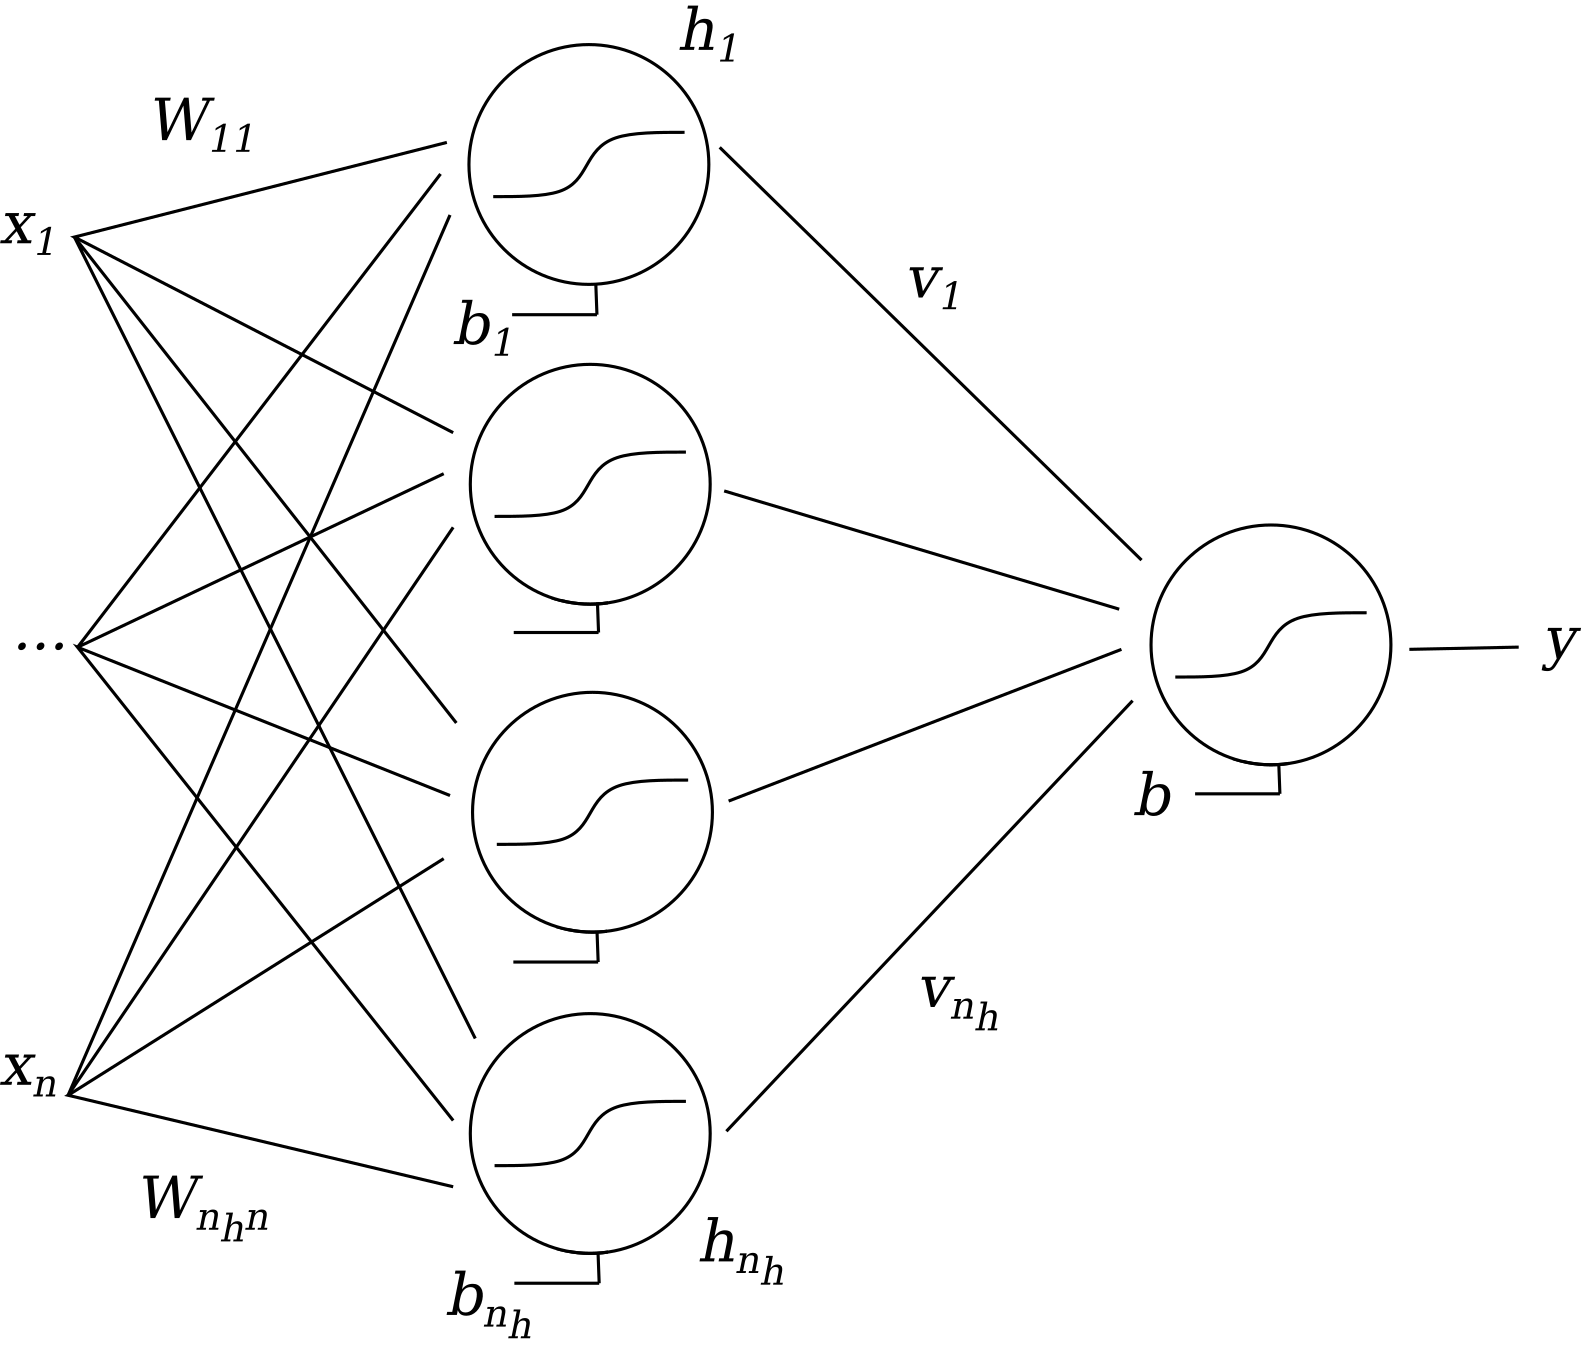
\includegraphics[width=0.6\linewidth]{graficos/propios/mlp.png}
    \caption{Arquitectura de una MLP típica \citep{bouzgou2012advanced}}
    \label{fig:mlp-eg}
\end{figure}

Tomando como ejemplo la figura \ref{fig:mlp-eg}, la salida de la neurona oculta $j$ es calculada procesando las entradas multiplicadas por sus respectivos pesos $w_{ij}$ y sumándole un bias $b_j$. Luego a este resultado le aplicamos una función de activación (ver fórmula \ref{eq:mlp-out}) que le permite a la red modelar relaciones no lineales en los datos. Esta función de activación suele ser la función logistica, la tangente hiperbólica o la función \ac{ReLU}. Para una comparación entre estas funciones ver figura \ref{fig:mlp-activation}

\begin{equation}
    \label{eq:mlp-out}
    h_j = f(b_j + \sum_{j=1}^{n_h} W_{ij} x_i)
\end{equation}

\begin{figure}[htbp]
    \centering
    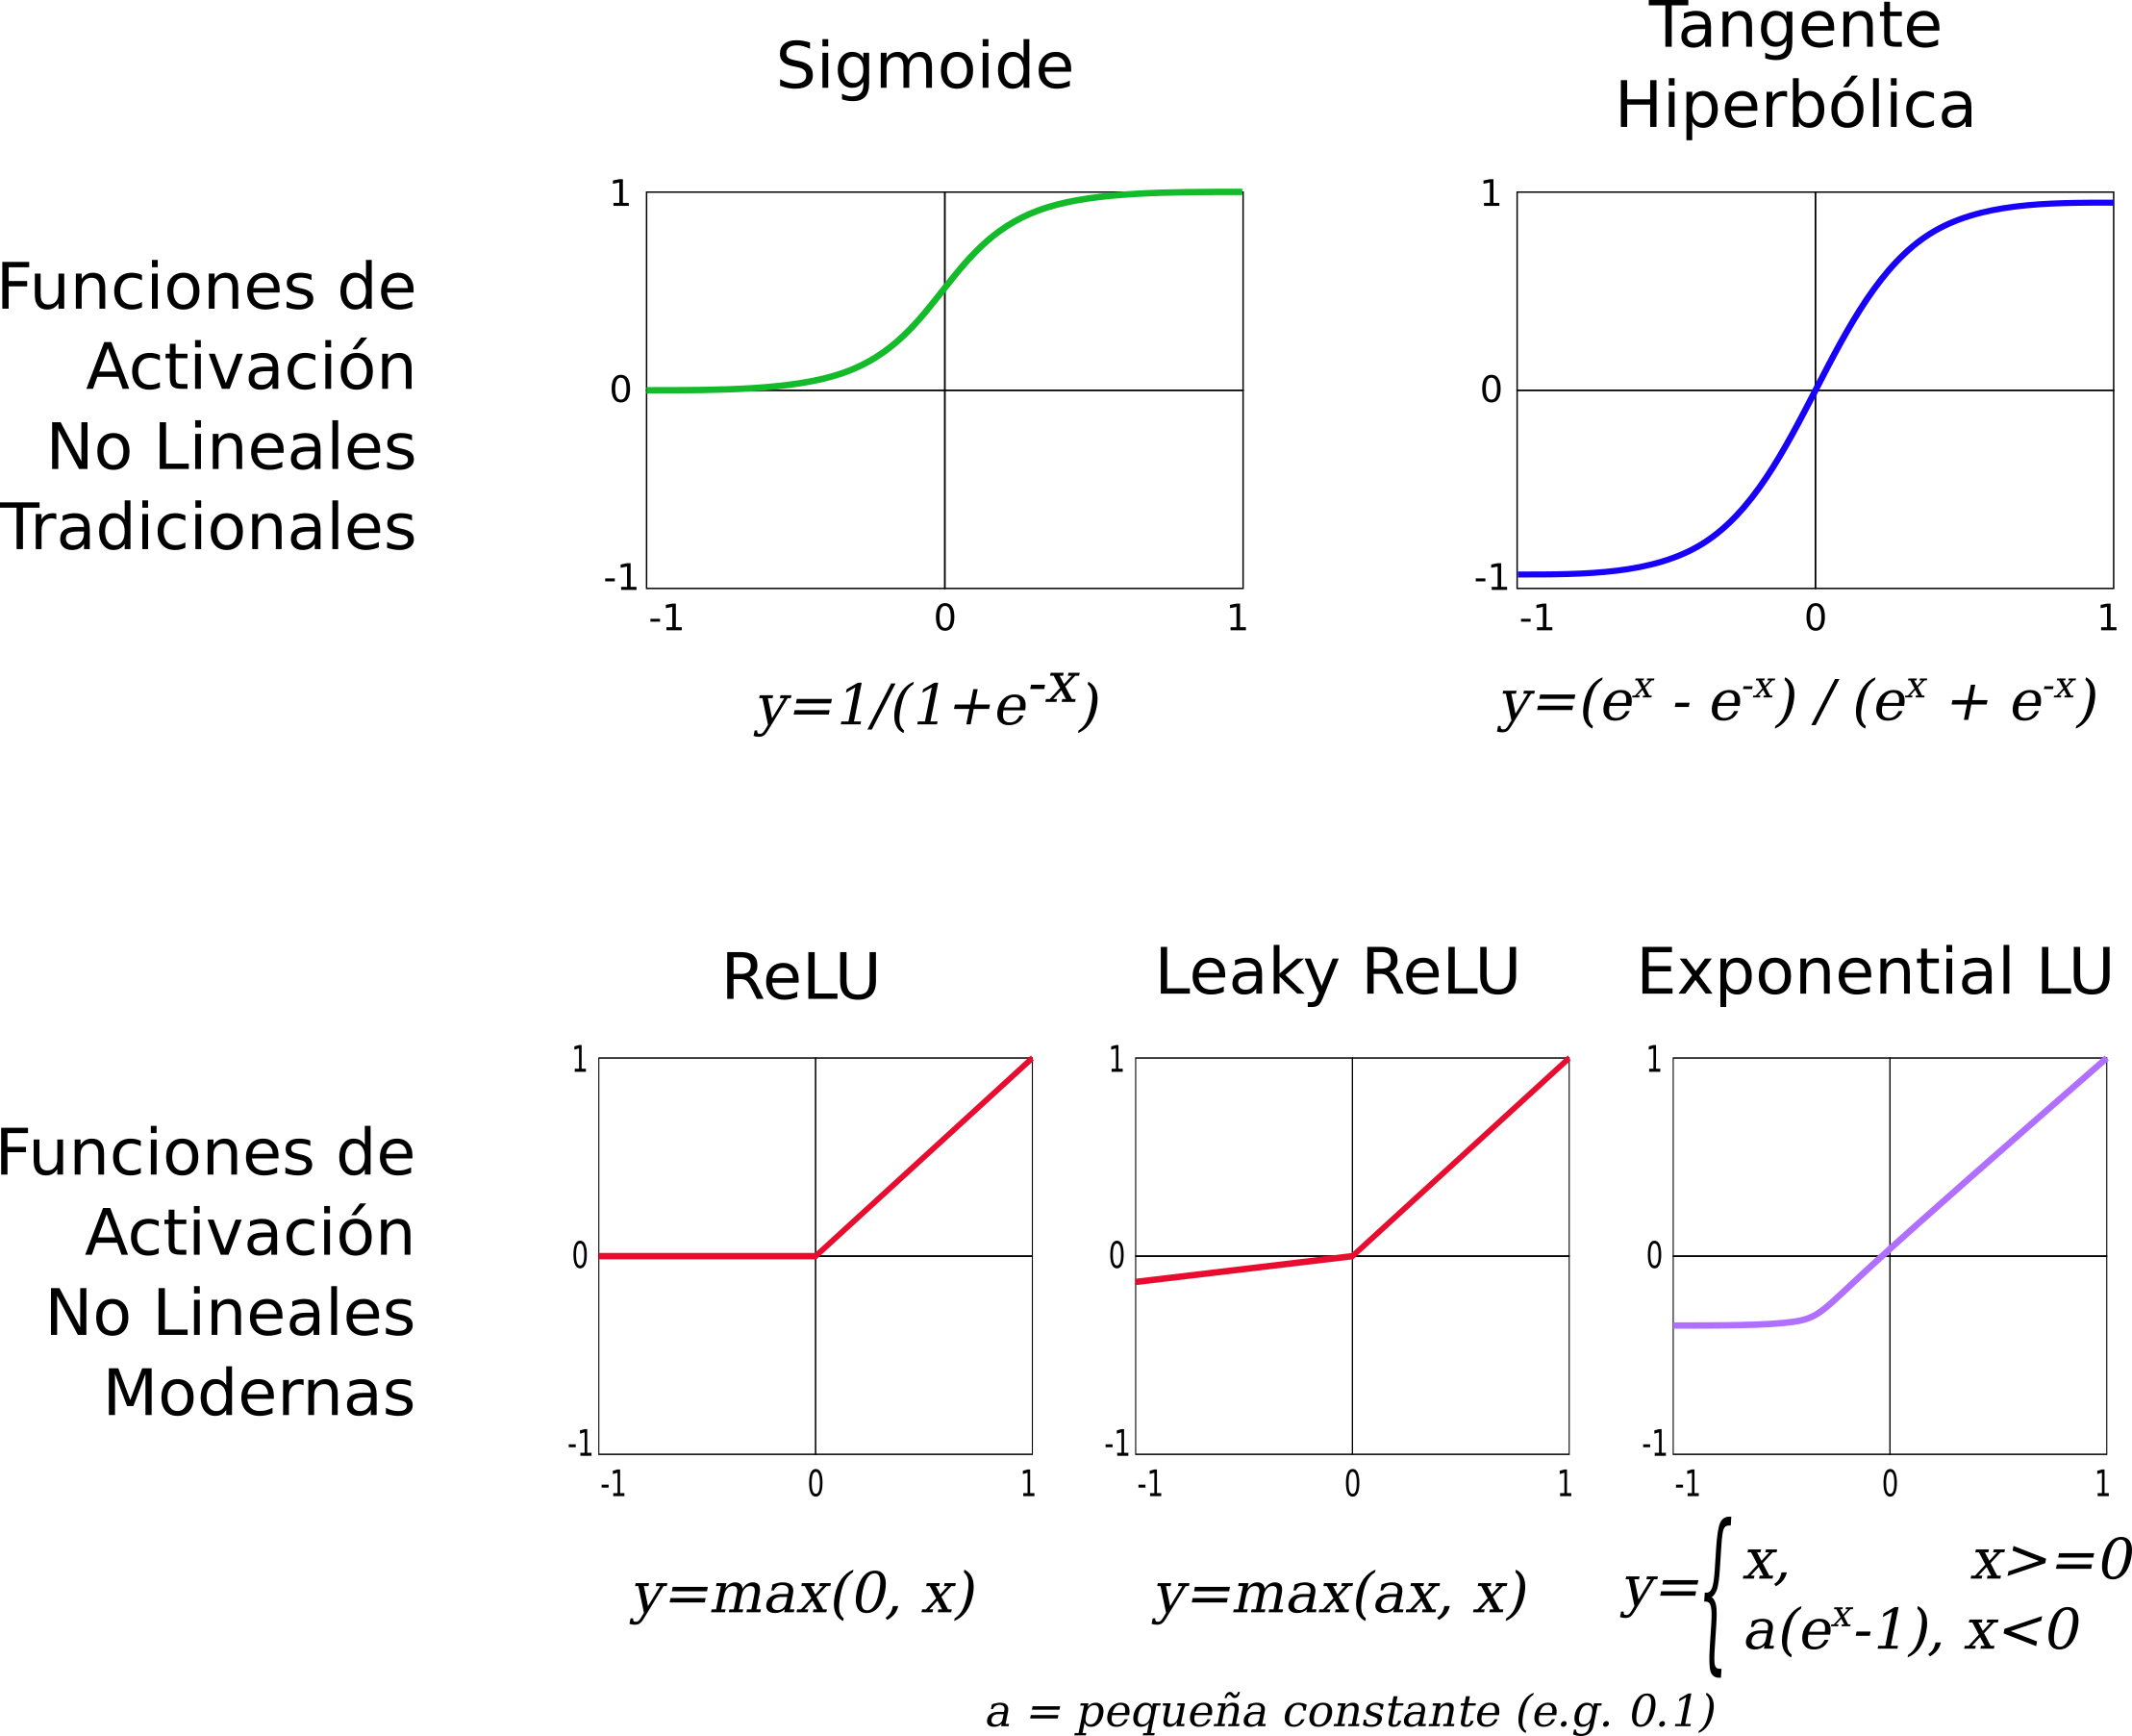
\includegraphics[width=0.8\linewidth]{graficos/propios/funciones_de_activacion.png}
    \caption{Funciones de activación \citep{sze2017efficient}}
    \label{fig:mlp-activation}
\end{figure}

\subsection{Deep Belief Network}

Es un tipo de red neuronal profunda, compuesta por múltiples capas de variables latentes (unidades ocultas), con conexiones entre las capas pero no entre unidades dentro de una misma capa.

El entrenamiento de esta red consiste en una etapa no supervisada seguida de otra supervisada. En la etapa no supervisada la \ac{DBN} aprende a reconstruir probabilísticamente sus entradas. Luego, se mejora la clasificación mediante la siguiente etapa de entrenamiento supervisado.

Las \ac{DBN} pueden ser vistas como la composición de redes simples no supervisadas tales como la \ac{RBM} o los autoencoders, donde la capa oculta de cada sub-red se convierte en la capa visible de la siguiente sub-red. Esta composición permite un proceso de entrenamiento no supervisado rápido capa por capa. Ver figura \ref{fig:dbn-train}.

\begin{figure}[htbp]
    \centering
    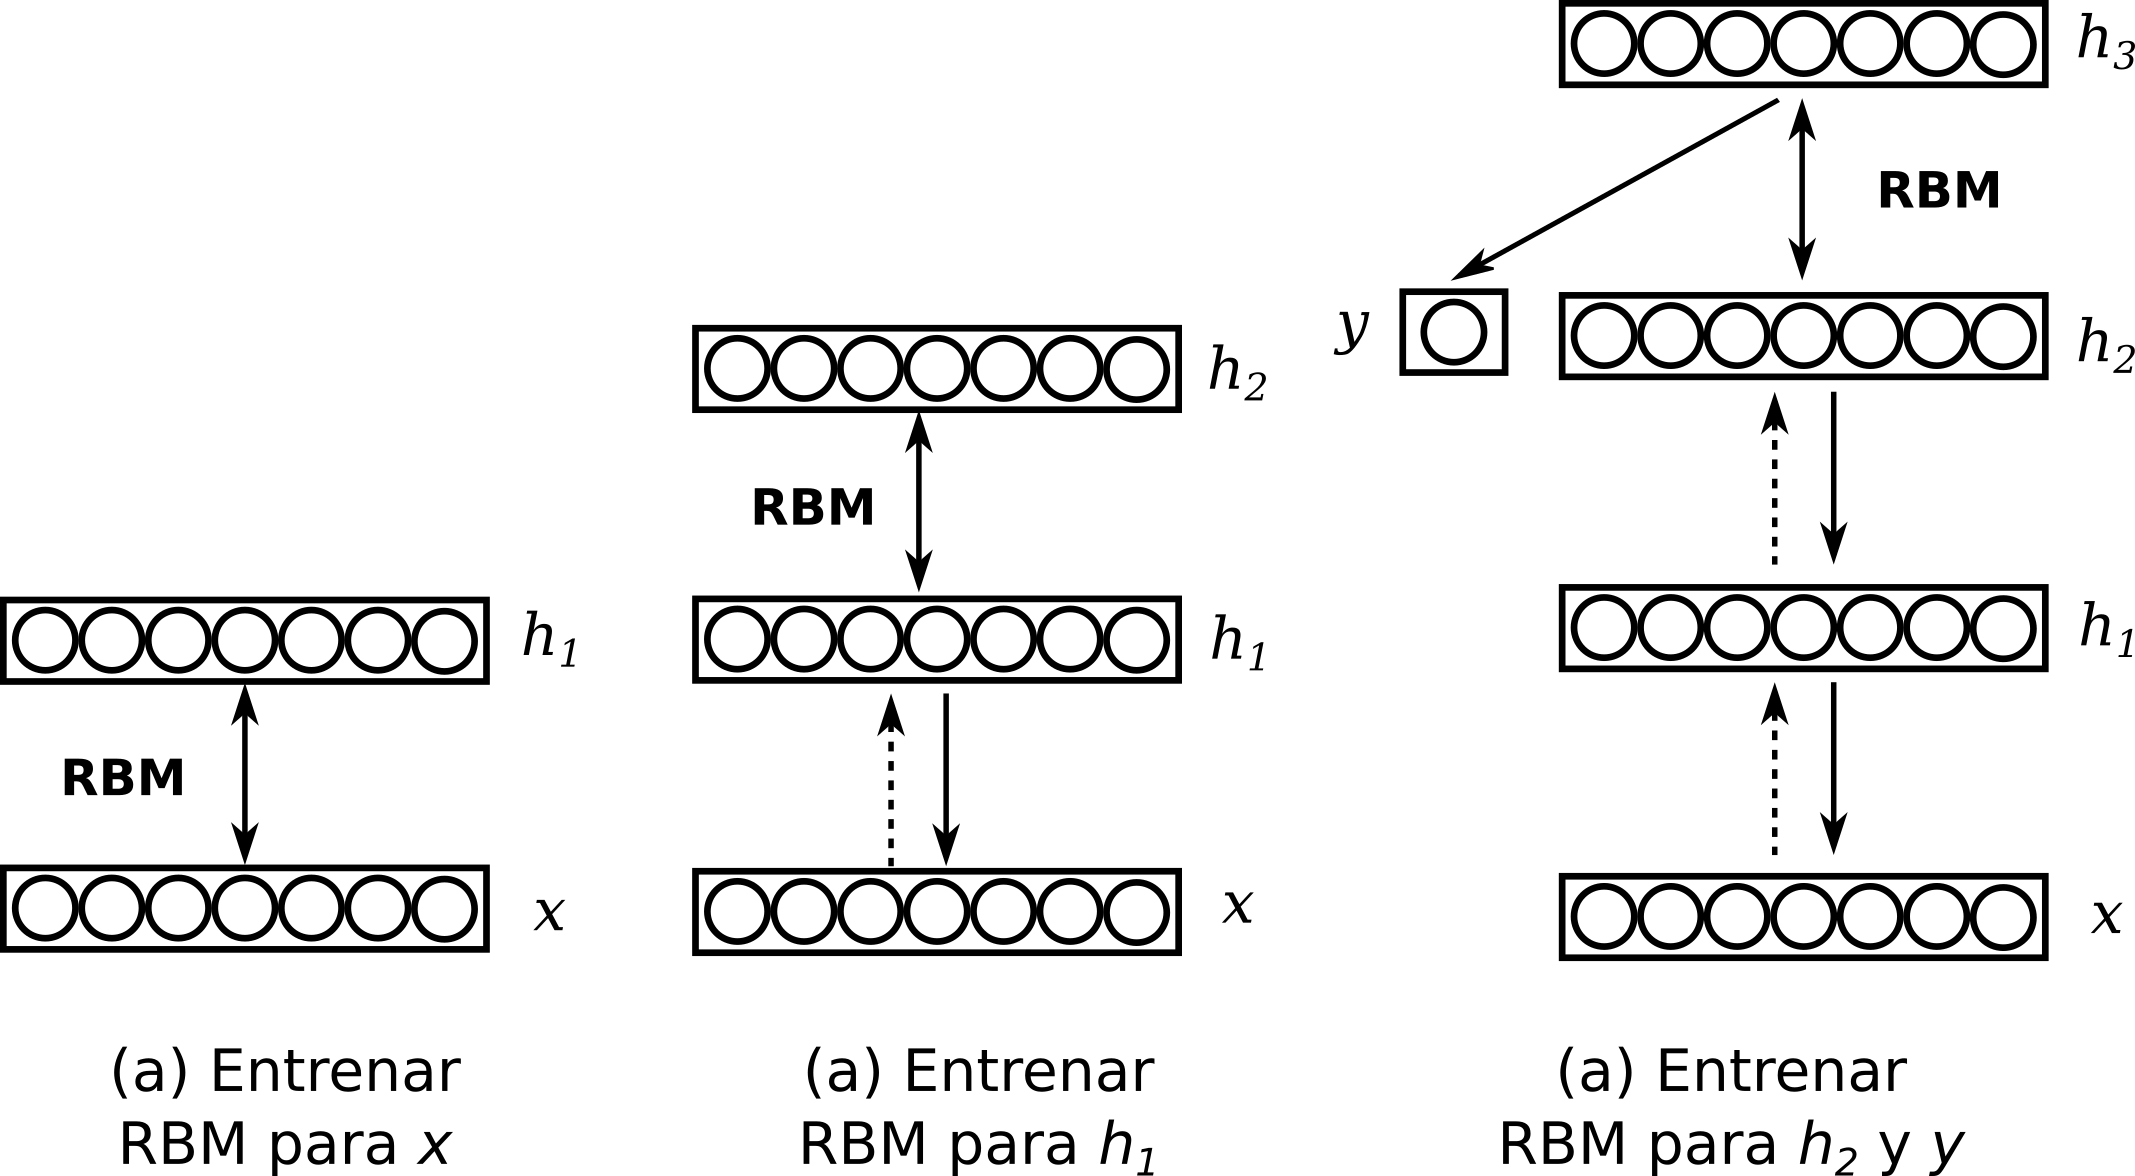
\includegraphics[width=0.9\linewidth]{graficos/propios/entrenamiento_dbn.png}
    \caption{Entrenamiento no supervisado de una DBN \citep{beysolow2017autoencoders}}
    \label{fig:dbn-train}
\end{figure}

\subsection{Support Vector Machine}

Es una familia de algoritmos de aprendizaje supervisado que pueden hacer clasificación y regresión \citep{cortes1995support}.

Funcionan construyendo un hiperplano o conjunto de hiperplanos en un espacio de dimensionalidad muy alta. Cada uno de estos hiperplanos está definido por el vector entre los dos puntos más cercanos de 2 clases diferentes, al que se llama vector de soporte. De esta manera se consigue separar a las clases con un margen máximo. La figura \ref{fig:svm-hiperplanos} ilustra esta forma de separación.

\begin{figure}[htbp]
    \centering
    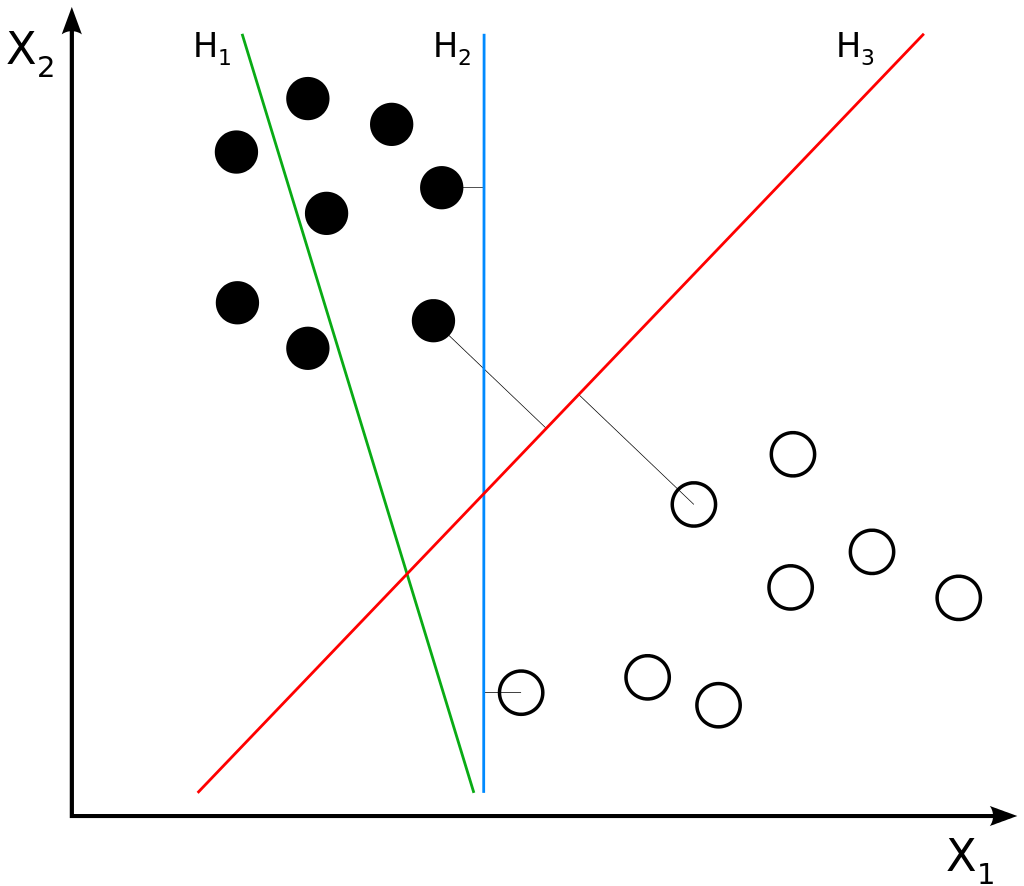
\includegraphics[width=0.4\linewidth]{graficos/svm_hiperplanos.png}
    \caption{Hiperplanos creados por una SVM \citep{wiki:svm_figure}}
    \label{fig:svm-hiperplanos}
    \par
    \small
    $H_1$ no separa las clases. $H_2$ las separa, pero solo con un margen pequeño. $H_3$ las separa con el margen máximo.
\end{figure}

Lamentablemente en las aplicaciones reales, las clases no suelen ser linealmente separables. Por eso existen las representaciones por medio de funciones de Kernel, que mapean el espacio de entradas $X$ a un espacio de características de mayor dimensionalidad, donde aumenta la capacidad computacional de las máquinas de aprendizaje lineal. Algunos tipos de función de Kernel son el Kernel Polinomial Homogéneo, el Kernel Perceptrón, la función de Base Radial Gaussiana y el Kernel Sigmoide \citep{cristianini2000introduction}.

Finalmente existe una versión de \ac{SVM} llamada \ac{LS-SVM}, que encuentra la solución resolviendo un conjunto de ecuaciones lineales en lugar de un problema convexo de programación cuadrática \citep{ak2002least}.

\subsection{Árbol de decisión}

Un árbol de decisión es un modelo simple de clasificación, se puede ver un ejemplo en la figura \ref{fig:dt-eg}. Cada nodo interno corresponde a una de las variables de entrada, y según el valor de esta se puede bajar a alguno de los nodos hijos. Cada hoja representa la predicción dada por los valores de la entrada representados por el camino desde la raíz hasta la hoja.

Los algoritmos para la construcción de árboles suelen trabajar de arriba hacia abajo, escogiendo una variable en cada paso que separa mejor los datos. Diferentes algoritmos usan diferentes métricas para definir una ``mejor separación de los datos''. Estos típicamente miden la homogeneidad de la variable objetivo en los subsets resultantes. Entre estos algoritmos tenemos la Impureza de Gini, la Ganancia de Información y la Reducción de la Varianza.

Entre las ventajas de los árboles de decisión tenemos que son fáciles de interpretar y requieren poca preparación de los datos. Sin embargo también tiene desventajas, como la tendencia al sobreajuste y la dificultad para aprender relaciones tipo XOR.

\begin{figure}[htbp]
    \centering
    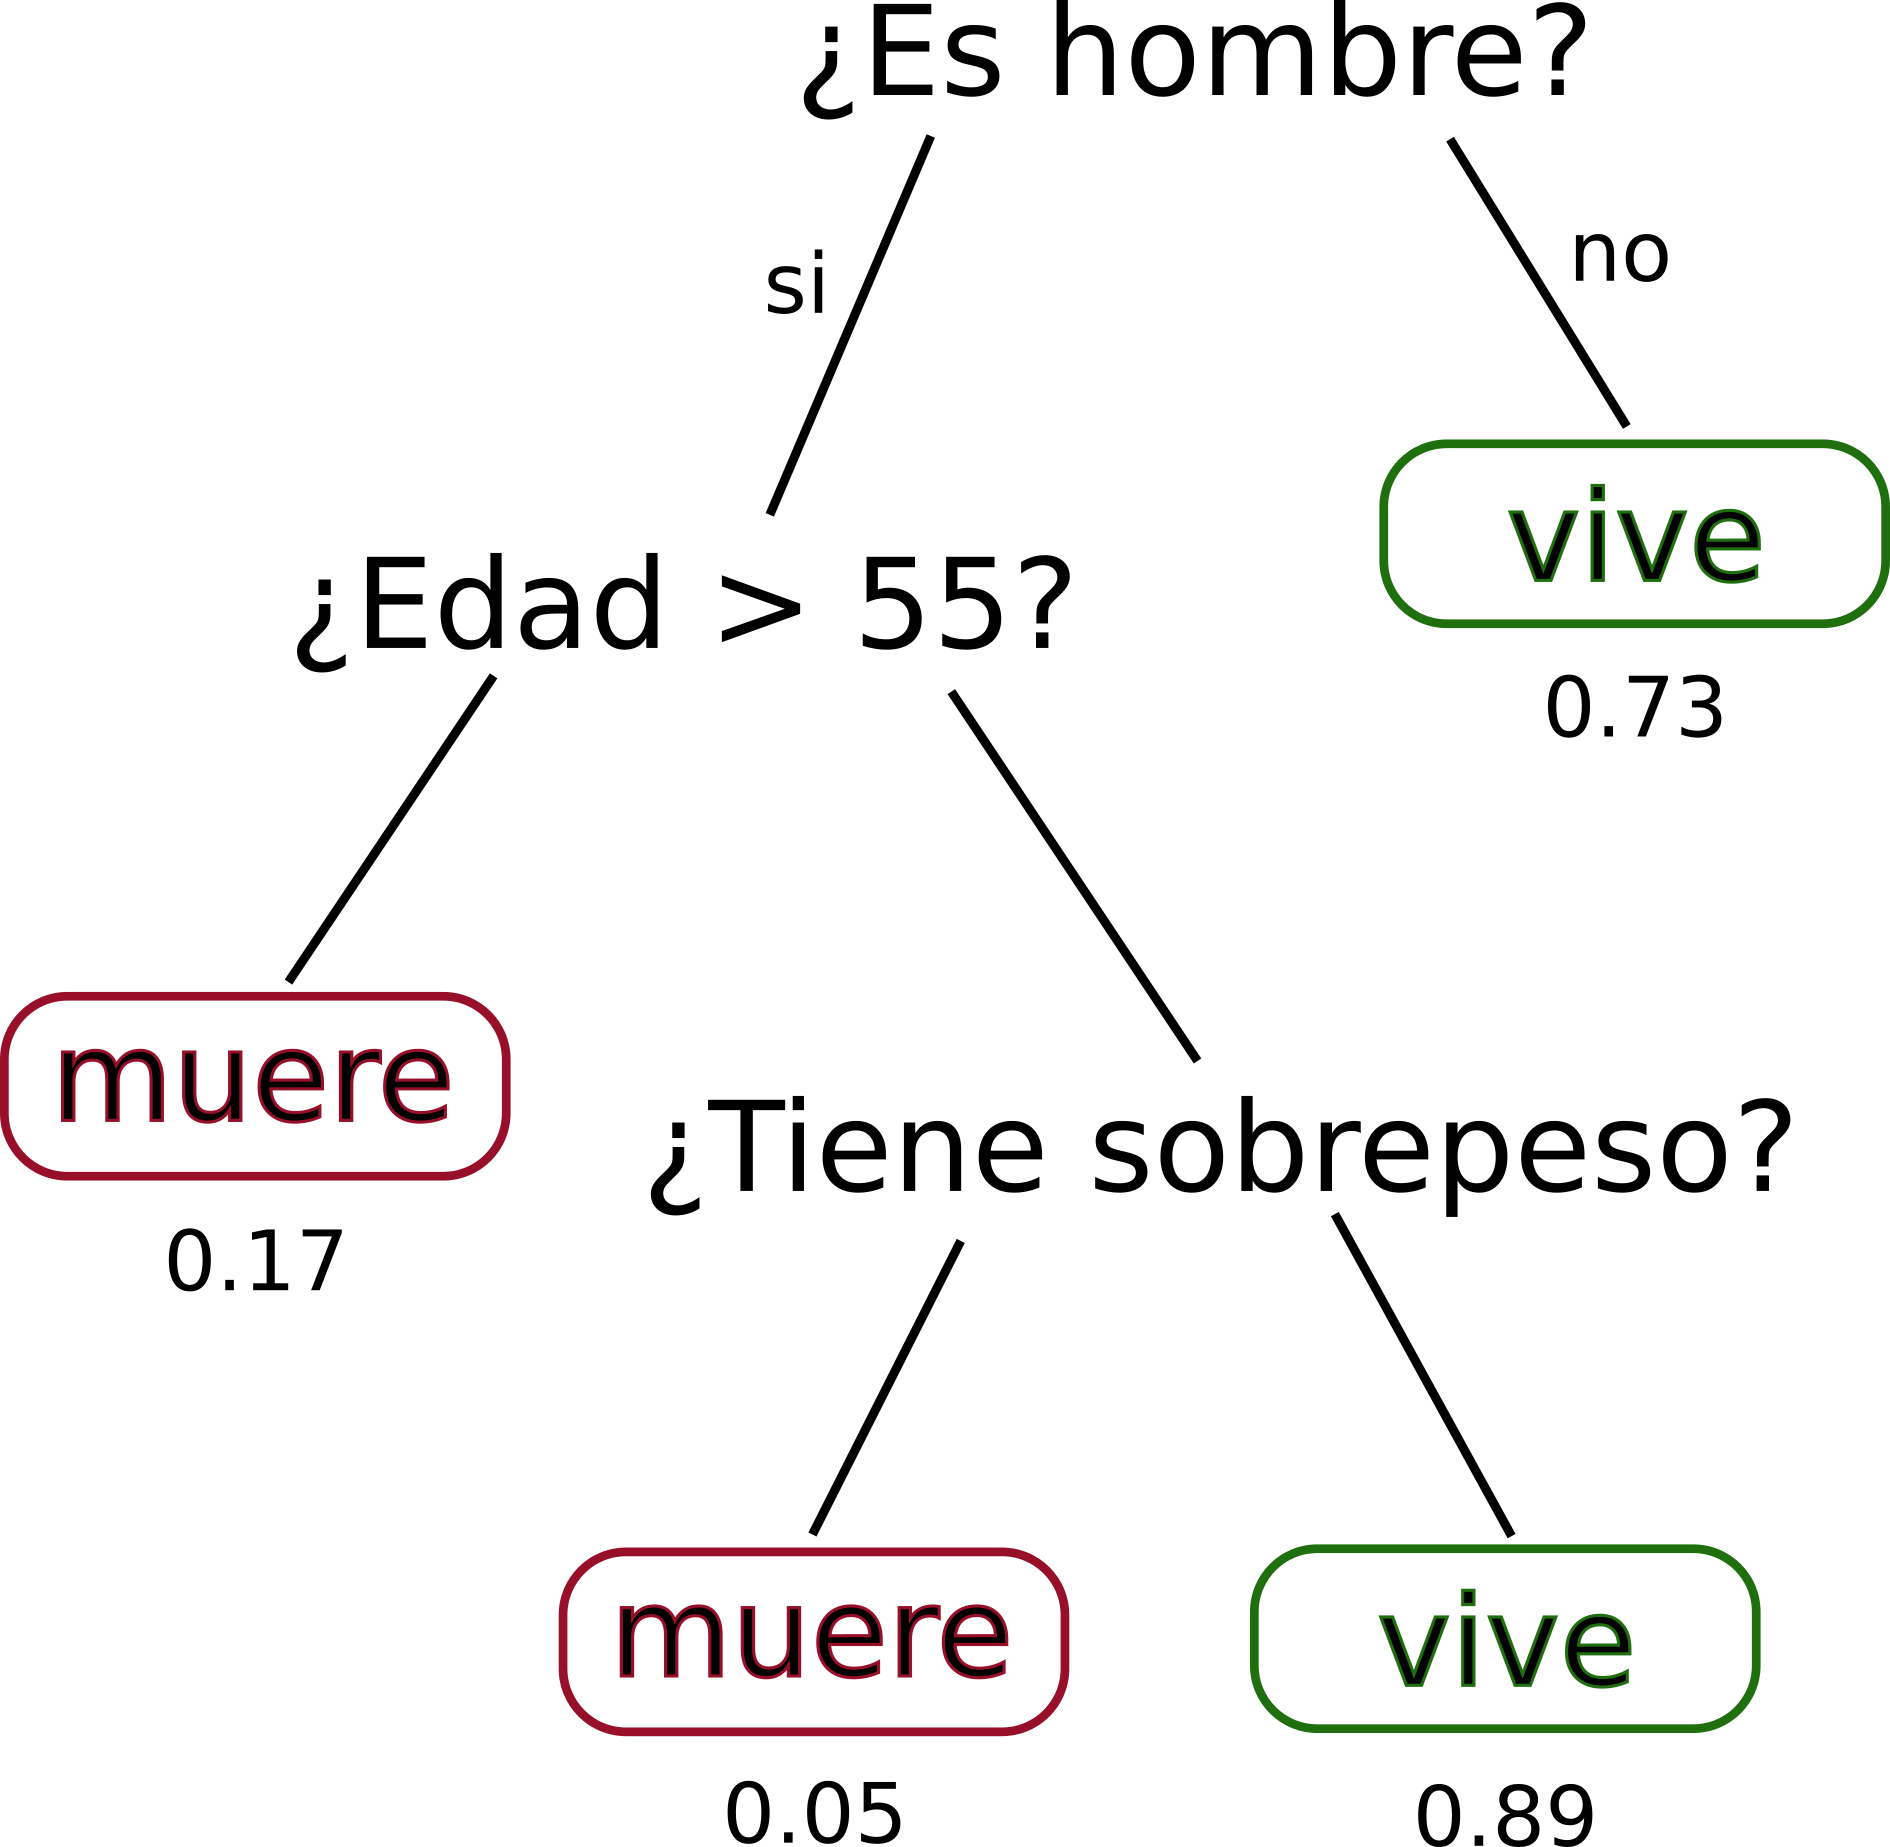
\includegraphics[width=0.4\linewidth]{graficos/propios/arbol_decision.png}
    \caption{Ejemplo de árbol de decisión}
    \label{fig:dt-eg}
\end{figure}

\section{Métodos de ensamble}

En el aprendizaje automático, los métodos de ensamble usan múltiples algoritmos de aprendizaje para obtener un mejor poder predictivo del que podría ser conseguido por cualquiera de los algoritmos constituyentes por sí solo.

Evaluar la predicción de un ensamble requiere más computaciones de las que requiere un modelo individual, así que los ensambles pueden ser imaginados como una manera para compensar algoritmos con un pobre aprendizaje realizando mucha computación adicional. Algoritmos rápidos como los árboles de decisión son comúnmente usados en los métodos de ensamble, sin embargo, otros algoritmos más lentos pueden beneficiarse de las técnicas de ensamble también.

\subsection{Random Forest}

Los árboles de decisión son algoritmos muy simples que permiten ver claramente la importancia de cada variable. Sin embargo, son proclives al sobreajuste, y se hace necesario limitar la profundidad de los árboles para mitigar este problema. Además, son muy inestables, ya que con pequeñas variaciones del conjunto de entrenamiento se puede generar un árbol completamente distinto. Esto es llamado varianza y se necesitan métodos como el bagging y el boosting para reducirla.

El funcionamiento básico del bagging dentro de Random Forest se puede resumir en pocos pasos (figura \ref{fig:rf}):

\begin{enumerate}
    \item Asumiendo que tenemos un conjunto de datos con 1000 instancias
    \item Creamos varias (e.g. 100) muestras aleatorias con repetición
    \item Entrenamos un árbol de decisión en cada muestra
    \item Dada una nueva instancia para clasificar, calculamos la predicción promedia de todos los árboles entrenados en el paso anterior
\end{enumerate}

\begin{figure}[htbp]
    \centering
    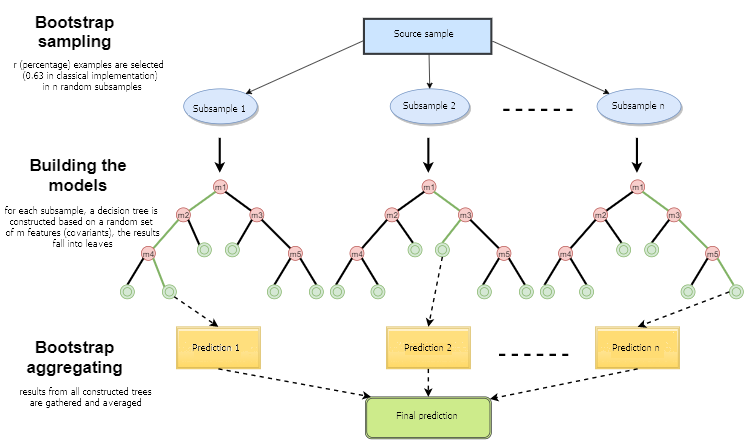
\includegraphics[width=\linewidth]{graficos/rf.png}
    \caption{Funcionamiento de Random Forest \citep{mql5:rf}}
    \label{fig:rf}
\end{figure}

Random Forest además incluye una mejora adicional conocida como Random Subspace. En lugar de entrenar los árboles de decisión con la totalidad de las variables, se escoge un subset aleatorio de variables y se entrena el árbol con ellas. Esto resulta en una mayor diversidad que generalmente produce un mejor modelo.

\subsection{XGBoost}

Boosting es un método similar a bagging que agrupa varios modelos débiles en un modelo fuerte. La diferencia con bagging es que no se crean muestras aleatorias con repetición, sino que se incrementa la exactitud del modelo de forma progresiva, haciendo que los módelos débiles se enfoquen más en las instancias mal clasificadas de los clasificadores anteriores. AdaBoost es un ejemplo simple de boosting que se puede resumir en el los siguientes pasos:

\begin{enumerate}
    \item Se escoge una muestra aleatoria del conjunto de entrenamiento
    \item Se entrena un clasificador débil con esta muestra y se clasifica todo el conjunto de entrenamiento
    \item A las instancias mal clasificadas se les da más peso para que tengan más probabilidad de aparecer en la siguiente muestra
    \item Se repite este proceso de manera que las instancias mal clasificadas reciben un mayor enfoque de los clasificadores subsiguientes
\end{enumerate}

Gradient boosting por otro lado, modela el problema de clasificación como una función de pérdida que debe ser minimizada. Cada nuevo clasificador débil es un paso más en la dirección negativa de la gradiente, con lo que se minimiza el error. Está tecnica es susceptible de sufrir sobre ajuste.

Finalmente, XGBoost es una implementación de Gradient Boosting en árboles de decisión creada por Tianqi Chen. La palaba extreme se refiere a la meta de ingeniería de aprovechar los recursos computacionales al límite, lo que provocó que su uso se expandiera rápidamente en la comunidad.

% \section{Recomendaciones generales de escritura}
% Un trabajo de esta naturaleza debe tener en consideración varios aspectos generales:

% \begin{itemize}
% \item Ir de lo genérico a lo específico. Siempre hay qeu considerar que el lector podría ser alguien no muy familiar con el tema 
% y la lectura debe serle atractiva.
% \item No poner frases muy largas. Si las frases son de mas de 2 líneas continuas es probable que la lectura sea dificultosa.
% \item Las figuras, ecuaciones, tablas deben ser citados y explicados {\bf antes} de que aparezcan en el documento.
% \item Encadenar las ideas. Ninguna frase debe estar suelta. Siempre que terminas un párrafo y hay otro a continuación, 
% el primero debe dejar abierta la idea que se explicará a continuación. Todo debe tener secuencia.
% \end{itemize}

\subsection{Método de ensamble para datos desbalanceados}


Muchos algoritmos de clasificación han demostrado un desempeño no óptimo en problemas con clases desbalanceadas \citep{batista2004study, mani2003knn, seiffert2010rusboost}.

El bagging es un método de aprendizaje de ensamble que podría resolver este problema si los clasificadores base fueran certeros y diversos \citep{breiman1996bagging}. Sin embargo, cada clasificador base dentro del bagging aún sufre del mismo problema, puesto que las instancias se muestrean proporcionalmente del conjunto original. Incluso si se balancean los datos antes de ejecutar los algoritmos de aprendizaje, se altera la distribución original y se hace overfitting.

El método de bagging propuesto \citep{sun2015novel} ataca un problema desbalanceado convirtiéndolo en varios problemas balanceados, lo cual incluye tres componentes: \textit{Balanceo del conjunto de datos, Modelamiento y Clasificación}. La figura \ref{fig:bagging-imbalanced} muestra los detalles.

\begin{figure}[htbp]
    \centering
    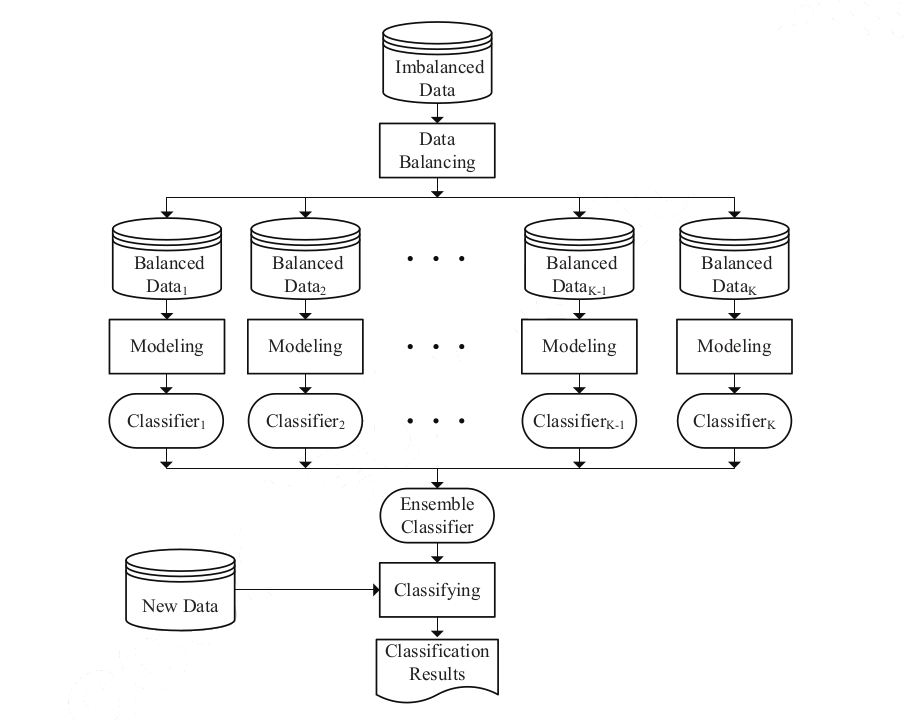
\includegraphics[width=\linewidth]{graficos/bagging_imbalanced.png}
    \caption{Método de bagging propuesto \citep{sun2015novel}}
    \label{fig:bagging-imbalanced}
\end{figure}

En este método, la clase mayoritaria genera varios subsets mediante muestreo sin repetición. Cada subset tiene un número de instancias igual a la clase minoritaria, y luego se combinan con esta. Así, se obtienen varios conjuntos de datos balanceados (Balanceo de los datos). Luego, cada conjunto se usa para crear un clasificador binario con un algoritmo específico (Modelamiento). Finalmente estos clasificadores binarios se combinan en un ensamble para clasificar nuevas instancias (Clasificación).

Esta combinación de los resultados de los clasificadores base se realiza mediante un promedio ponderado por la inversa de la distancia de la instancia a clasificar con el subset utilizado. De esta manera, los subsets más parecidos a la nueva instancia tendrán un mayor peso en la decisión final.


\section{Evaluación de los modelos}

\subsection{Exactitud, Precisión y Exhaustividad}

Para entender estos conceptos necesitamos conocer primero a la matriz de confusión. Esta es una herramienta que permite la visualización del desempeño de un algoritmo de clasificación. Cada columna de la matriz representa el número de predicciones de cada clase, mientras que cada fila representa a las instancias en la clase real. Uno de los beneficios de las matrices de confusión es que facilitan ver si el sistema está confundiendo dos clases. Se puede ver un ejemplo en la figura \ref{fig:confussion}.

\begin{figure}[htbp]
    \centering
    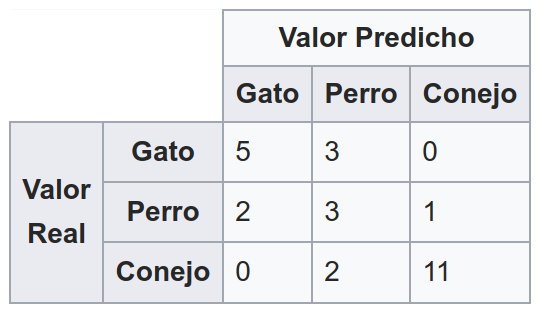
\includegraphics[width=0.5\linewidth]{graficos/confussion_matrix.png}
    \caption{Ejemplo de matriz de confusión}
    \label{fig:confussion}
\end{figure}

Cuando el problema de clasificación sólo tiene 2 clases, la matriz de confusión se parece más a la figura \ref{fig:confussion2}.

\begin{figure}[htbp]
    \centering
    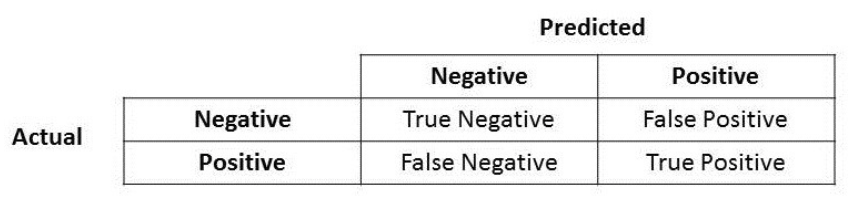
\includegraphics[width=0.8\linewidth]{graficos/confussion_matrix_2.png}
    \caption{Ejemplo de matriz de confusión con dos clases}
    \label{fig:confussion2}
\end{figure}

A partir de esta matriz se pueden definir formalmente la exactitud, precisión y exhaustividad como se ve en la fórmula \ref{eq:accuracy-prec-rec}.

\begin{equation}
    \label{eq:accuracy-prec-rec}
\begin{split}
    \text{Exactitud}  &= \frac{\text{verdaderos positivos} + \text{verdaderos negativos}}{\text{verdaderos positivos} + \text{falsos positivos} + \text{verdaderos negativos} + \text{falsos negativos}} \\\\
    \text{Precisión} &= \frac{\text{verdaderos positivos}}{\text{verdaderos positivos} + \text{falsos positivos}} \\\\
    \text{Exhaustividad}    &= \frac{\text{verdaderos positivos}}{\text{verdaderos positivos} + \text{falsos negativos}} 
\end{split}
\end{equation}

De forma más intuitiva podemos definirlos de la siguiente manera:

\begin{description}
    \item [Exactitud] Porcentaje de clasificaciones correctas
    \item [Precisión] De aquellos clasificados como positivos, cuántos son realmente positivos
    \item [Exhaustividad] De la población total de positivos, cuántos clasificó como positivos nuestro modelo
\end{description}

Aunque en el ámbito de la calificación crediticia lo normal sea que la clase positiva sean las personas morosas, si invertimos esta situación haciendo que la clase positiva sean las personas que pagan su crédito, entonces la precisión y la exhaustividad se vuelven métricas muy útiles, con significados muy prácticos:

\begin{description}
    \item [Precisión] De las personas que el modelo clasificó como buenos pagadores, cuántos realmente pagan sus préstamos. En otras palabras esta métrica se convierte en $1 - \text{\% de morosidad}$. Y representa muy bien el riesgo crediticio del modelo.
    \item [Exhaustividad] Del universo de buenos pagadores, cuántos pueden ser capturados con este modelo. Está métrica tiene una incidencia directa en el costo de adquisión de los clientes.
\end{description}

En otras palabras, el balance entre precisión y exhaustividad se convierte en el balance entre el riesgo que se quiere asumir y el costo de adquisición de los clientes y el tamaño del mercado. En cambio el concepto de Exactitud no tiene una incidencia directa en algún aspecto del problema, además de que no es una buena métrica a utilizar en conjuntos desbalanceados.

Pongamos un ejemplo extremo de desbalance, donde sólo una persona de cada 1000 no paga su crédito. Un modelo que simplemente trate de maximizar la exactitud puede aprender erróneamente a clasificar a todos como si pertenecieran a la clase mayoritaria, obteniendo así una exactitud de 0.999.

En estos casos de desbalance tan extremo también la precision y la exhaustividad se ven afectadas, cosa que se soluciona invirtiendo las clases, i.e. haciendo que 0 sean las personas que pagan y 1 las personas que no pagan adecuadamente. Con esta disposición, y con el mismo ejemplo de tener 1 moroso en 1000 personas, la precisión sería de 0 y la exhaustividad también, indicando que nuestro modelo no tiene poder predictivo.

\subsection{Curva ROC y Area bajo la curva (AUC)}

Las métricas vistas en la sección anterior tienen un inconveniente: es necesario encontrar un punto de corte para poder calcularlas. La curva ROC en cambio, evalúa y compara el desempeño de los algoritmos sin necesidad de escoger un punto de corte.

La curva ROC grafica la relación entre la razón de verdaderos positivos y la razón de falsos positivos según se varía el umbral de discriminación. Mientras esta curva se acerque más a la esquina superior izquiera, mejor será la clasificación.

El \ac{AUC} es una medida que nos permite comparar diferentes curvas fácilmente. Funciona calculando el área debajo de la curva ROC, tal como su nombre lo indica. Ver figura \ref{fig:eg-roc}.

\begin{figure}[htbp]
    \centering
    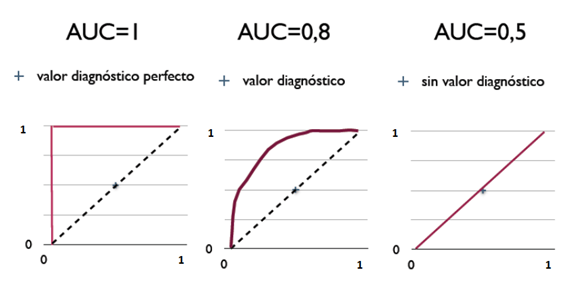
\includegraphics[width=0.8\linewidth]{graficos/eg_roc.png}
    \caption{Ejemplo de curvas ROC \citep{wiki:roc_figure}}
    \label{fig:eg-roc}
\end{figure}

Finalmente cabe mencionar que pueden existir dos curvas ROC diferentes que tengan la misma área bajo la curva. Por eso no se puede descartar el uso de las curvas ROC totalmente, ya que dependiendo de a qué se le quiera dar más importancia, se escogerá una curva y otra. Tarea que es imposible solamente observando el \ac{AUC}.

%\section{Repeated-N cross fold validation}


%\section{Pruebas de hipótesis estadísticas}

%\subsection{Pairwise comparison}
%\subsection{Analysis of variance}
%\subsection{Friedman test}
%\subsection{Friedman test with post-hoc test}
%Demšar, J. (2006). Statistical comparisons of classifiers over multiple data sets. Journal of Machine Learning
%Research, 7, 1-30.
%\subsection{Press Q statistic}

\section{Trabajo relacionado}

Actualmente hay mucho trabajo científico buscando mejorar los sistemas de calificación crediticia mediante diferentes técnicas.

En \citep{sohn2016technology} se propone una regresión logística difusa para explotar mejor atributos de evaluación linguísticos. Los resultados son que efectivamente se mejora el desempeño respecto a una regresión logística normal. En \citep{bahnsen2014example} se propone una regresión logística que usa una matriz de costo dependiendo de cada ejemplo. Los resultados subrayan la importancia de usar los costos financieros reales, ya que se logran mejoras significativas en términos de ahorro de dinero.

Por otro lado en \citep{zhao2015investigation} se aplica una \ac{MLP} que se trata de optimizar mediante (i) la mejora de la distribución de los datos usando un método llamado Average Random Choosing, (ii) probando diferentes tamaños de conjuntos de train-test-validation y (iii) encontrar el número óptimo de neuronas ocultas. Los resultados son bastante alentadores y los autores claman que se pueden utilizar incluso fuera del dominio de los puntajes de crédito.

En el área de aprendizaje profundo también se ha hecho progreso. Particularmente en \citep{luo2017deep} se hace uso de una \ac{DBN} que se compara con algoritmos más populares de calificación crediticia como \ac{LR}, \ac{MLP} y \ac{SVM}. Los modelos son aplicados en un conjunto de contratos CDS XR 14 (sin reestructuración) y los resultados arrojan que la \ac{DBN} tiene la mejor exactitud y AUC.

En \citep{huang2007credit} se usan tres estrategias para construir modelos híbridos de \ac{SVM}, las pruebas se ejecutan con dos conjuntos de datos crediticios de la UCI. Comparados con redes neuronales, programación genética y clasificadores de árboles, los \ac{SVM} tienen una exactitud idéntica con relativamente pocas características. Adicionalmente, al combinar algoritmos genéticos con \ac{SVM}, se puede realizar simultáneamente la selección de variables y la optimización de parámetros del modelo. 

En otro estudio \citep{harris2015credit} se introduce el uso de \ac{CSVM} para calificación crediticia. Este algoritmo resolvería algunas limitaciones \ac{SVM}, particularmente se centra en el costo computacional en conjuntos grandes, logrando niveles de clasificación similares mientras se mantiene un costo computacional bajo.

En \citep{malekipirbazari2015risk} se propone una clasificación basada en \ac{RF}. Se utilizan los datos de préstamos peer2peer Lending Club, y los resultados indican que los métodos basado en \ac{RF} superan los score crediticios del FICO así como los propios scores de LC.

Además se presentan algunos métodos nuevos, como el \ac{RF} paralelo de \citep{van2016novel}. Donde al integrar el modelo en el proceso de selección de variables se mejora la exactitud promedio obteniendo un 76.2\%.

En \citep{xia2017boosted} y \citep{bhatia2017credit} se experimenta con \ac{XGBoost}. En el primer artículo se centra en el ajuste de los parámetros del modelo, mientras que el segundo hace una comparación más amplia con otros modelos como \ac{LDA} y \ac{RF}.

Los préstamos \ac{P2P} son una opción para tomar préstamos de personas individuales sin utilizar un banco o una entidad financiera tradicional. En \citep{zhang2016research} se usa un conjunto de datos \ac{P2P} para construir un modelo basado en árboles de decisión fusionando datos de los medios de comunicación sociales. En \citep{zang2014credit} también se usa un conjunto de datos \ac{P2P}, perteneciente a Lending Club. Se aplica una \ac{MLP} y se obtienen resultados favorables. Para terminar con \ac{P2P}, en \citep{tan2018deep} se utiliza una red neuronal profunda para modelar los riesgos en competencia, el del prestamista y el del prestatario, este sería el primer lugar donde se prueba dicho concepto obteniendo un desempeño interesante en las inversiones.

En \citep{nanni2009experimental} se prueban varios clasificadores de ensamble en los datos de crédito Alemán y Australiano. Dichos clasificadores ensamblados mejoran el desempeño de sus respectivos clasificadores base. En \citep{brown2012experimental} se hace un estudio comparativo de varios modelos en cinco conjuntos de datos distintos. Se hace un énfasis especial en el desbalanceo de la datos, pues se hace un undersampling de la clase minoritaria para pronunciar el desbalance cada vez más y evaluar como se van comportando los modelos en cada caso. Los resultados son que \ac{RF} y clasificadores de Gradient Boosting se desempeñan bien incluso en conjuntos de datos altamente desbalanceados. Finalmente en \citep{wang2012two} se proponen dos estrategias de ensamble para árboles, que luego se comparan con cinco clasificadores base y cuatro clasificadores de ensamble, obteniendo resultados competitivos.

En conclusión, hasta la fecha se ha venido realizando un trabajo muy diverso. El área de calificación crediticia es un área muy fértil, pero aún quedan muchas potenciales mejoras por realizarse.

\section{Consideraciones Finales}

Ahora que tenemos una idea clara de cómo funcionan los clasificadores base, los ensambles y los métodos de evaluación; podemos pasar a explicar los conjuntos de datos utilizados, la metodología y los experimentos realizados.
 %Inserta el capítulo 2
\chapter{Experimentos}

%El título del capítulo es flexible de acuerdo a cada tesis. Algunos títulos sugeridos podrían ser:
%\begin{itemize}
%\item El algoritmo X: nuestra propuesta.
%\item La técnica Y
%\end{itemize}
%Este título debe de estar ade acuerdo con el asesor del tema. Consúltelo en su sala de clase.

En este capítulo explicaremos la información necesaria y los procedimientos seguidos para llevar a cabo la experimentación. En primer lugar se explicarán los conjuntos de datos que servirán de base y referencia para los experimentos; luego se detallarán algunos detalles de la metodología; y finalmente se explicarán los experimentos a seguir.

\section{Conjuntos de datos}

Los conjuntos de datos que serán utilizados como casos de prueba son los siguientes:

\begin{description}
	\item[Apurata] Conjunto de datos privado de la \textit{fintech} peruana con el mismo nombre
	\item[Lending Club] Conjunto de datos público de la mayor \textit{fintech} de préstamos \ac{P2P} en EE.UU.
	\item[Crédito Alemán] Conjunto de datos público de entidades bancarias Alemanas
\end{description}

Una mejor comparación entre estos conjuntos se puede encontrar en la tabla \ref{tab:dataset-comparison}

\begin{table}
	\centering
	\caption{Conjunto de datos utilizados}
	\label{tab:dataset-comparison}
	\begin{tabular}{@{}lll@{}}
	\toprule
	\textbf{Apurata}	& \textbf{Lending Club}		& \textbf{Crédito Alemán}	\\
	\midrule
	Perú (2016-2018)	& E.E.U.U (2007-2015)		& Alemania (1994)			\\
	100 - 1,000 PEN		& 1000 - 35,000 USD			& 1,000 - 20,000 EUR		\\
	1 - 9 semanas		& 36 - 60 meses				& 6 - 60 meses				\\
	626 observaciones	& 194,208 observaciones		& 1000 observaciones		\\
	33 atributos		& 46 atributos				& 24 atributos				\\
	\bottomrule
	\end{tabular}
\end{table}

Como se puede apreciar, todos los conjuntos se componen de pocas características, ninguno de ellos supera las 50. Los conjuntos de datos de Apurata y del Crédito Alemán además son pequeños respecto a la cantidad de instancias, con 1000 o menos.

También se cumple que los 3 conjuntos de datos son desbalanceados, ya que la clase de ``Moroso", representa el 15\% para Apurata, 24\% para Lending Club y el 30\% para Crédito Alemán.

Por otro lado, los 3 conjuntos también poseen diferencias importantes entre sí que enriquecen su estudio. Apurata y Lending Club son \textit{fintech} que utilizan diferentes criterios de los de los bancos para seleccionar su información. Los conjuntos de Crédito Alemán y Lending Club registran créditos que se realizan por montos más altos y a un mayor plazo que los de Apurata. Los periodos de tiempo y los países abarcados por los conjuntos de datos también son únicos, y finalmente Lending Club tiene bastante más instancias que los otros 2 conjuntos.

Los conjuntos de Crédito Alemán y Lending Club son considerados referenciales en sus respectivos sub-dominios, ya que hay varios estudios que los utilizan para realizar sus experimentos. Entre los que usan los datos de Lending Club tenemos \citep{malekipirbazari2015risk, zhang2016research, zang2014credit, tan2018deep}. Y entre los que usan los datos del Crédito Alemán tenemos \citep{harris2015credit, nanni2009experimental, brown2012experimental, wang2012two}.

\section{Metodología}

Para el preprocesamiento de la información, se eliminaron las variables con más del 50\% de información faltante, luego se eliminaron las filas con información faltante. A las variables resultantes se les convirtió a variables numéricas; y finalmente se hizo una normalización entre -1 y 1.

La interpretación de la variable $y$ se hizo de la siguiente manera: 1 para los buenos pagadores y 0 para los malos.

Para la selección de parámetros se realizó un grid-search con un ajuste fino manual al final. Sobre el desbalanceo de los datos, no se tomó ningún procedimiento especial.

Para evaluar el desempeño de los modelos se hizo 10-fold validation 10 veces en Apurata y en el Crédito Alemán y 1 sola vez en Lending Club, ya que tiene abundantes datos. Finalmente se extrajo el promedio de todas las mediciones como la medición final.

Las métricas utilizas son la exactitud, la precisión, la exhaustividad y el \ac{AUC}. La métrica que se buscó optimizar fue el \ac{AUC}. Para las otras métricas se tuvo que seleccionar un punto de corte óptimo, que se escogió tratando de optimizar la exactitud, de modo que los resultados son comparables con el estado del arte.

\section{Experimentos}

En esta sección se describirán los experimentos llevados a cabo.

\subsection{Experimento 1}

El primer paso es hacer una comparación entre los clasificadores individuales y los \ac{ECDD}. El objetivo de este experimento es verificar si efectivamente el desempeño mejora individualmente por cada clasificador, sin hacer una comparación transversal entre clasificadores de distintas familias.

En este experimento también evaluaremos la posibilidad de usar un algoritmo de aprendizaje profundo: \ac{DBN}.

\subsection{Experimento 2}

En este experimento compararemos los \ac{ECDD} con dos algoritmos de \textit{bagging} usados ampliamente en la actualidad: \ac{RF} y \ac{XGBoost}. El objectivo de este experimento es verificar que el método de \ac{ECDD} es competitivo con otros métodos de ensamble del estado del arte, sin el sesgo de haber usado una metodología diferente para el entrenamiento y la evaluación de los modelos.

\subsection{Experimento 3}

Finalmente en el experimento 3 compararemos los resultados obtenidos por nuestros \ac{ECDD} con los resultados obtenidos en otros estudios del estado del arte que usan los mismos conjuntos de datos. El objetivo de este experimento es ratificar que los resultados son válidos para el estado del arte usando dos conjuntos de datos referenciales.
 %Inserta el capítulo 3
\chapter{Pruebas y Resultados}

\section{Proceso 1} %%%%%%%%%%%%%%%%%%%%%%%%%%%%%%%%%%%%%%%%%%%%%%%%%%%%%%%%%%%%%%%%

Los resultados del proceso 1 se pueden ver en las Tablas \ref{tab:apurata-proc1}, \ref{tab:lc-proc1} y \ref{tab:german-proc1}.

Se ve que en el \ac{AUC}, la precisión y la exactitud mejoran en todos los clasificadores. Particularmente el AUC se incrementa un promedio de 4.30 en Apurata, 2.80 en Lending Club y 1.62 en el Crédito Alemán.

La exhaustividad baja en la mayoría de modelos, ya que existe un balance entre la precisión y la exhaustividad. Y ya que se trató de optimizar la exactitud, indirectamente se optimizó la precisión, de forma que la exhaustividad cayó un poco.

Se desprende también que la potencial mejora que podemos obtener con el método de ensamble para datos desbalanceados depende del clasificador base y del conjunto de datos sobre el cuál se aplica.

Si analizamos cuál fue el algoritmo base más afectado por el \ac{ECDD}, vemos claramente que el árbol de decisión es el ganador. Esto se debe a que individualmente el árbol de decisión es muy sensible al ruido y fácilmente hace overfitting. Sin embargo al ponerlo dentro de un ensamble, su capacidad de generalizar mejora. De hecho es la misma razón por la que los algoritmos de ensamble más poderosos actualmente usan árboles de decisión como su clasificador base.

\subsection{Sobre el aprendizaje profundo}

El caso de la \ac{DBN} es particular. En primer lugar, ajustar los parámetros del modelo resulta complejo, porque son varios parámetros y porque al ser poca información el modelo presenta una tendencia a caer en overfitting. Esto se observa al tener un desempeño impecable con los datos de entrenamiento, pero un desempeño muy inferior con los datos de prueba.

Luego de ajustar cuidadosamente los parámetros de la mejor forma posible, el poder predictivo no es mejor que otros clasificadores base, específicamente es muy similar al de una \ac{MLP} simple. Esto se puede explicar con la baja dimensionalidad de los datos y la poca cantidad de instancias; ya que no se explota la capacidad de reducción de dimensionalidad del modelo y tampoco se hace un entrenamiento adecuado por la escasez de datos.

En conclusión, este clasificador no es adecuado para este problema, y al ser bastante complejo ya de por sí, no se le creó una versión ensamblada.


\begin{table}[]
\centering
\caption{Proceso 1 con conjunto de datos de Apurata}
\label{tab:apurata-proc1}
\begin{tabularx}{0.75\textwidth}{|l|Y Y Y Y|}
				\hline
				& AUC		& Precisión	& Exhaustividad	& Exactitud	\\
				\hline
LR				& 70.02		& 89.25		& 96.35			& 82.78		\\
ECDD-LR			& 72.56		& 89.76		& 95.96			& 82.86		\\
				\hline
MLP				& 68.13		& 88.96		& 91.86			& 80.30		\\
ECDD-MLP		& 70.61		& 89.64		& 92.30			& 80.61		\\
				\hline
AD				& 61.75		& 86.84		& 98.06			& 83.71		\\
ECDD-AD			& 68.81		& 89.42		& 92.93			& 80.73		\\
				\hline
SVM				& 66.56		& 89.33		& 87.65			& 78.39		\\
ECDD-SVM		& 71.70		& 89.81		& 94.44			& 82.04		\\
				\hline
DBN				& 67.80		& 88.04		& 91.76			& 79.84		\\
				\hline
\end{tabularx}
\end{table}


\begin{table}[]
\centering
\caption{Proceso 1 con conjunto de datos de LendingClub}
\label{tab:lc-proc1}
\begin{tabularx}{0.75\textwidth}{|l|Y Y Y Y|}
				\hline
				& AUC		& Precisión	& Exhaustividad	& Exactitud	\\
				\hline
LR				& 73.36		& 77.83		& 95.40			& 75.05		\\
ECDD-LR			& 73.34		& 77.55		& 96.23			& 74.85		\\
				\hline
MLP				& 74.87		& 78.29		& 95.74			& 75.71		\\
ECDD-MLP		& 75.67		& 79.09		& 94.07			& 75.82		\\
				\hline
AD				& 75.52		& 77.94		& 92.86			& 75.34		\\
ECDD-AD			& 80.34		& 81.88		& 89.50			& 78.05		\\
				\hline
SVM				& 73.53		& 77.42		& 97.29			& 75.03		\\
ECDD-SVM		& 74.41		& 78.29		& 95.91			& 75.00		\\
				\hline
DBN				& 75.01		& 78.56		& 94.92			& 75.72		\\
				\hline
\end{tabularx}
\end{table}


\begin{table}[]
\centering
\caption{Proceso 1 con conjunto de datos Alemán}
\label{tab:german-proc1}
\begin{tabularx}{0.75\textwidth}{|l|Y Y Y Y|}
				\hline
				& AUC		& Precisión	& Exhaustividad	& Exactitud	\\
				\hline
LR				& 71.45		& 81.77		& 99.32			& 78.92		\\
ECDD-LR			& 71.50		& 81.84		& 98.83			& 78.68		\\
				\hline
MLP				& 69.36		& 81.26		& 98.76			& 78.78		\\
ECDD-MLP		& 71.61		& 82.44		& 97.08			& 79.00		\\
				\hline
AD				& 66.86		& 79.48		& 99.85			& 78.35		\\
ECDD-AD			& 71.82		& 82.71		& 96.02			& 79.20		\\
				\hline
SVM				& 67.54		& 80.79		& 97.28			& 79.12		\\
ECDD-SVM		& 71.49		& 82.27		& 97.88			& 79.35		\\
				\hline
DBN				& 66.84		& 80.07		& 97.98			& 78.24		\\
				\hline
\end{tabularx}
\end{table}


\section{Proceso 2} %%%%%%%%%%%%%%%%%%%%%%%%%%%%%%%%%%%%%%%%%%%%%%%%%%%%%%%%%%%%%%%%

Los resultados del proceso 2 se pueden ver en las Tablas \ref{tab:apurata-proc2}, \ref{tab:lc-proc2} y \ref{tab:german-proc2}. Para comparar estos resultados se realizó una prueba de T de Student desapareada.

El modelo ECDD-LR \textit{(M=$72.56$, SD=$3.21$)} comparado al modelo \ac{RF} \textit{(M=$69.23$, SD=$3.13$)} demostró un \ac{AUC} significativamente mejor, $t(198)=7.47, p=.0001$.

Se observa que el desempeño de los \ac{ECDD} es ligeramente superior al desempeño de \ac{RF} y \ac{XGBoost}. Si comparamos la mejora obtenida por el mejor \ac{ECDD} respecto al mejor entre RF y XGBoost; vemos que el AUC en Apurata incrementa 3.33, en Lending Club mejora 0.50 y en Crédito Alemán aumenta en 0.06.

Lamentablemente no es posible extrapolar estos resultados a otros dominios donde también hayan conjuntos de datos desbalanceados, ya que los conjuntos de datos crediticios además del desbalance poseen otras características que podrían no cumplirse en otros dominios, como la estacionalidad de los datos, la baja cantidad de features y la información parcialmente oculta. De modo que no podemos afirmar que estos \ac{ECDD} son universalmente mejores que Random Forest y XGBoost.

Otra observación interesante es el buen desempeño que obtiene la Regresión Logística en el conjunto de Apurata. Esto podría indicar que la información es linealmente separable y los otros modelos sufren de un poco de overfitting, razón por la cuál su desempeño no es óptimo.

Finalmente, el \ac{ECDD} de árboles de decisión obtiene resultados muy buenos consistentemente en Lending Club y el Crédito Alemán, lo que sugiere que si los datos no son linealmente separables, entonces este modelo tiene un gran poder predictivo. Probando una vez más que usar los árboles de decisión como base para algoritmos de ensamble tiene muy buenos resultados.

\begin{table}[]
\centering
\caption{Proceso 2 con conjunto de datos de Apurata}
\label{tab:apurata-proc2}
\begin{tabularx}{0.75\textwidth}{|l|Y Y Y Y|}
				\hline
				& AUC		& Precisión	& Exhaustividad	& Exactitud	\\
				\hline
ECDD-LR			& 72.56		& 89.76		& 95.96			& 82.86		\\
ECDD-MLP	 	& 70.61		& 89.64		& 92.30			& 80.61		\\
ECDD-SVM	 	& 71.70		& 89.81		& 94.44			& 82.04		\\
ECDD-AD			& 68.81		& 89.42		& 92.93			& 80.73		\\
				\hline
RF		 		& 69.23		& 89.37		& 94.57			& 81.66		\\
XGB				& 67.91		& 89.31		& 89.92			& 78.75		\\
				\hline
\end{tabularx}
\end{table}


\begin{table}[]
\centering
\caption{Proceso 2 con conjunto de datos de LendingClub}
\label{tab:lc-proc2}
\begin{tabularx}{0.75\textwidth}{|l|Y Y Y Y|}
				\hline
				& AUC		& Precisión	& Exhaustividad	& Exactitud	\\
				\hline
ECDD-LR			& 71.50		& 81.84		& 98.83			& 78.68		\\
ECDD-MLP		& 71.61		& 82.44		& 97.08			& 79.00		\\
ECDD-SVM		& 71.49		& 82.27		& 97.88			& 79.35		\\
ECDD-AD			& 71.82		& 82.71		& 96.02			& 79.20		\\
				\hline
RF				& 71.32		& 82.18		& 97.23			& 78.79		\\
XGB				& 70.68		& 81.89		& 98.56			& 78.81		\\
				\hline
\end{tabularx}
\end{table}


\begin{table}[]
\centering
\caption{Proceso 2 con conjunto de datos Alemán}
\label{tab:german-proc2}
\begin{tabularx}{0.75\textwidth}{|l|Y Y Y Y|}
				\hline
				& AUC		& Precisión	& Exhaustividad	& Exactitud	\\
				\hline
ECDD-LR			& 73.34		& 77.55		& 96.23			& 74.85		\\
ECDD-MLP		& 75.67		& 79.09		& 94.07			& 75.82		\\
ECDD-SVM		& 74.41		& 78.29		& 95.91			& 75.00		\\
ECDD-AD			& 80.34		& 81.88		& 89.50			& 78.05		\\
				\hline
RF				& 79.82		& 80.84		& 92.01			& 76.22		\\
XGB				& 80.28		& 81.43		& 91.66			& 78.93		\\
				\hline
\end{tabularx}
\end{table}


\section{Proceso 3} %%%%%%%%%%%%%%%%%%%%%%%%%%%%%%%%%%%%%%%%%%%%%%%%%%%%%%%%%%%%%%%%

Los resultados del proceso 3 se pueden ver en las Tablas \ref{tab:lc-proc3} y \ref{tab:german-proc3}. Sólo tenemos resultados para Lending Club y el Cŕedito Alemás puesto que Apurata es un conjunto de datos privado que es usado de forma inédita en este trabajo.

Es importante notar que al haber seguido procesos diferentes, los resultados de diferentes estudios tienen una variación más alta que si se hubieran hecho las comparaciones usando los mismo procesos. Es por esto que las conclusiones del proceso 2 son tan importantes.

Los modelos utilizados en los estudios referenciales son bastante diversos, abarcando modelos lineales y no lineales, de árboles y redes neuronales, llegando incluso a incluir redes neuronales profundas.

Si vemos los resultados a grandes rasgos, se observa que los \ac{ECDD} son efectivamente competitivos con el estado del arte. Con lo cuál podemos concluir que aplicar este método de ensamble para conjuntos de datos desbalanceados al dominio de los puntajes de crédito puede tener resultados bastante interesantes e incluso tener un poder predictivo ligeramente mayor a otros algoritmos más extendidos en la comunidad científica.


\begin{table}[]
\centering
\caption{Proceso 3 con conjunto de datos de LendingClub}
\label{tab:lc-proc3}
\begin{tabularx}{\textwidth}{|l|Y Y l|}
				\hline
				& AUC			& Exactitud		& Ref.									\\
				\hline
ECDD-LR			& 71.50			& 78.68			&										\\
ECDD-MLP		& 71.61			& 79.00			&										\\
ECDD-SVM		& 71.49			& 79.35			&										\\
ECDD-AD			& 71.82			& 79.20			&										\\
				\hline
RF				& 71.00			& 78.00			& Malekipirbazari, M.et al (2015)		\\
SVM				& 62.00			& 63.30			& Malekipirbazari, M.et al (2015)		\\
AD				& -				& 81.22			& Zhang, Y. Et al (2016)				\\
NN				& -				& 77.40			& Zhang, Y. Et al (2016)				\\
MLP				& -				& 78.60			& Zang, D. et al (2015)					\\
crDNN			& 72.55			& -				& Tan, F. et al (2018)					\\
LR				& 71.52			& -				& Tan, F. et al (2018)					\\
mcDNN			& 70.88			& -				& Tan, F. et al (2018)					\\
CRSA			& 69.30			& -				& Tan, F. et al (2018)					\\
				\hline
\end{tabularx}
\par
\small
Las investigaciones utilizadas para la comparación son en orden: \citep{malekipirbazari2015risk, zhang2016research, zang2014credit, tan2018deep}
\end{table}


\begin{table}[]
\centering
\caption{Proceso 3 con conjunto de datos Alemán}
\label{tab:german-proc3}
\begin{tabularx}{\textwidth}{|l|Y Y l|}
						\hline
						& AUC		& Exactitud	& Ref.									\\
						\hline
ECDD-LR					& 73.34		& 74.85		&										\\
ECDD-MLP				& 75.67		& 75.82		&										\\
ECDD-SVM				& 74.41		& 75.00		&										\\
ECDD-AD					& 80.34		& 78.05		&										\\
						\hline
SVM-linear				& 69.13		& 78.70		& Harris, T. (2015)						\\
SVM-RBF					& 69.53		& 78.00		& Harris, T. (2015)						\\
CSVM-RBF				& 69.23		& 77.10		& Harris, T. (2015)						\\
MLP						& 78.09		& 75.20		& Nanni, L. \& Lumini, A. (2009)		\\
Rand Subsp LMNC			& 78.47		& 73.93		& Nanni, L. \& Lumini, A. (2009)		\\
Bagging MLP				& 79.32		& 75.33		& Nanni, L. \& Lumini, A. (2009)		\\
Class Switch MLP		& 78.62		& 73.93		& Nanni, L. \& Lumini, A. (2009)		\\
Rotat Forest MLP		& 79.39		& 75.00		& Nanni, L. \& Lumini, A. (2009)		\\
Lin LS-SVM				& 81.90		& -			& Brown, I. \& Mues, C. (2012)			\\
Random Forests			& 80.00		& -			& Brown, I. \& Mues, C. (2012)			\\
RS-Bagging AD			& -			& 78.36		& Wang, G. et al. (2012)				\\
Bagging-RS AD			& -			& 78.52		& Wang, G. et al. (2012)				\\
						\hline
\end{tabularx}
\par
\small
Las investigaciones utilizadas para la comparación son en orden: \citep{harris2015credit, nanni2009experimental, brown2012experimental, wang2012two}
\end{table}

 %Inserta el capítulo 4
\chapter{Conclusiones y Trabajos Futuros}\label{chap:conclusiones}

%En primer lugar debes escribir las conclusiones generales de tu trabajo. evita escribirlas en forma de viñetas. Simplemente utiliza texto continuo.

Hemos visto que en el área de credit scoring hay abundante investigación, pero que no se ha explotado lo suficiente características del dataset crediticio típico, como el desbalanceo de los datos, el cuál se trato de explotar en este trabajo para obtener los mejores resultados posibles.

Se vio que al aplicar un algoritmo recientemente propuesto de ensamble para conjuntos de datos desbalanceados con varias familias de clasificadores base, se mejora el poder predictivo en prácticamente la totalidad de los casos. Sin embargo esta mejora depende del dataset en cuestión y el modelo base que se esté utilizando.

El caso del aprendizaje profundo, y específicamente de la \ac{DBN} es particular, porque la complejidad de ajustar los parámetros del modelo es elevada y el beneficio obtenido no lo justifica. Y debido a que este clasificador ya es bastante complejo de por sí no se le creó una versión ensamblada.

Por otro lado, al comparar los resultados de los \ac{ECDD} con otros métodos de ensamble del estado del arte, específicamente \ac{RF} y \ac{XGBoost}, vemos que se consigue una pequeña mejora, lo cuál es muy alentador.

Lamentablemente estos resultados no se pueden extrapolar a otros dominios debido a las particularidades de los datasets crediticios.

Al igual que con otros algoritmos de ensamble en estado del arte, el Decision Tree fue el clasificador base que mejor se adaptó al método de ensamble para datasets desbalanceados.

Finalmente cuando comparamos nuestros resultados con el estado del arte actual, observamos que este método de ensamble para datasets desbalanceados puede producir modelos competitivos, lo cuál refuerza la idea de profundizar la investigación en explotar las características inherentes a la data crediticia.

\section{Problemas encontrados}

El procesamiento de la información es costoso en términos de tiempo del investigador. Hay que entender las variables para poder transformarlas o eliminarlas de forma efectiva.

Hay demasiadas combinaciones de modelos y parámetros, y esto se puede complicar aún más si agregamos métodos de bagging, por lo que se requiere muchas ejecuciones de los modelos para encontrar los parámetros mas adecuados. Esto, al igual que el punto anterior es costoso en términos de tiempo del investigador.

Los resultados de una sóla ejecución pueden no ser confiables, esto es fácilmente detectable si al ejectuar varias veces las pruebas los resultados no son estables. Esto es especialmente susceptible en datasets pequeños, como los que se trabajan en esta investigación.

A pesar de que el mejor método para comparar algoritmos sea el AUC; ya que no depende de la selección de un punto de corte y es insensible al desbalanceo de las clases; otros estudios del estado del arte insisten en utilizar otras métricas sub-óptimas como el accuracy. De modo que uno se ve forzado a usar estas mismas métricas para poder comparar sus resultados con el estado del arte de forma mas o menos efectiva.

% La segunda  parte de ests capítulo corresponde a los problemas encontrados. esta seccion es muy importante para que los siguientes estudiantes que hagan algo en esta línea no cometan los mismos errores y tu tesis sea un buen peldaño para avanzar más rápido.

\section{Recomendaciones}

Si la limpieza de la data no es parte de la investigación, hay que procurar tomar datasets ya pre-procesados.

Si el dataset es pequeño y los resultados cambian con cada ejecución de las pruebas, hay que utilizar cross validation con repetición. El número de repeticiones se puede escoger a mano hasta que los resultados sean estables. Basta probar que los resultados sean estables con un modelo simple como \ac{LR} y podemos asumir que van a seguir siendo estables con modelos más complejos.

Usar datasets heterogéneos permite obtener conclusiones más generalizables, y hacer una mejor comparación que no esté tan sesgada por características particulares de ciertos datasets.

%En esta sección el tesista debe reflejar que la tesis ha permitido adquirir nuevos conocimientos que podrían servir para guiar otros trabajos en el futuro.

\section{Trabajo futuro}

En este trabajo vimos que atender algunas de las características de los datasets de credit scoring ayudan a mejorar el desempeño de los modelos. Por lo tanto los trabajos futuros se pueden enfocar en explotar las características que no fueron cubiertas en esta investigación, como lo son la sensibilidad al costo, y la estacionalidad de la data.

% En base a los puntos anteriores es recomendable que tu tesis también sugiera trabajos futuros. Esta sección es esecialmente útil para otras ideas de tesis.

%Todo este capítulo no debe ser más de unas 4 páginas. %Inserta el capítulo 5

%%%%%%%%%%%%%%%%%%%%%%%%%%%%%%%%%%%%%%%%%%%%%%%%%%%%%%%%%%%%%%%%%%%%%%

\bibliographystyle{apalike}
\bibliography{tesis}
\addcontentsline{toc}{chapter}{Bibliografía}
\end{document}
